\documentclass{beamer}
\usetheme{Boadilla} % Clean structure
\useinnertheme{circles} % Dots for sections
\useoutertheme{miniframes} % Header nav with section progress
\setbeamertemplate{navigation symbols}{} % Remove nav icons

\usepackage[utf8]{inputenc}
\usepackage{amsmath, amsfonts, graphicx, booktabs, hyperref}
\usepackage{tikz, caption}
\usepackage{booktabs}
% Custom colors
\definecolor{DeepBlue}{RGB}{0,51,102}
\setbeamercolor{title}{fg=DeepBlue}
\setbeamercolor{institute}{fg=DeepBlue}
\setbeamercolor{frametitle}{fg=DeepBlue}
\setbeamercolor{structure}{fg=DeepBlue}
\setbeamercolor{item}{fg=DeepBlue}

% Frame title underline
\setbeamertemplate{frametitle}{
    \insertframetitle\\
    \vspace{-0.3cm}
    \color{DeepBlue}\rule{\linewidth}{0.2mm}
    \vspace{0.3cm}
}

% Footer with long title and date
\setbeamertemplate{footline}
{
  \leavevmode%
  \hbox{%
  \begin{beamercolorbox}[wd=.20\paperwidth,ht=2.25ex,dp=1ex,center]{author in head/foot}%
    {\fontsize{6}{6} \selectfont Anushka Mukherjee}
  \end{beamercolorbox}%
  \begin{beamercolorbox}[wd=.60\paperwidth,ht=2.25ex,dp=1ex,center]{title in head/foot}%
    \usebeamerfont{title in head/foot}{\fontsize{6}{6}\selectfont Modeling Household Carbon Footprints - August 19, 2025}
  \end{beamercolorbox}%
  \begin{beamercolorbox}[wd=.20\paperwidth,ht=2.25ex,dp=1ex,right]{date in head/foot}%
    {\fontsize{6}{6} \selectfont \insertframenumber{} / \inserttotalframenumber}\hspace*{1em}
  \end{beamercolorbox}}%
  \vskip0pt%
}

% Title info
\title[Modeling Household Carbon Footprints]{Modeling Household Carbon Footprints:\\ Methods, Metrics, and Estimation Frameworks}
\author[Anushka Mukherjee]{Anushka Mukherjee}
\institute[University of Bonn]{University of Bonn}
\date[July 2025]{August 19, 2025}

\begin{document}

% Title slide
\begin{frame}
  \titlepage
\end{frame}

% Table of contents
\begin{frame}{Overview}
  \tableofcontents
\end{frame}

% -------------------
\section{Introduction}
\begin{frame}{Motivation}
\vspace{-2.0em}
\footnotesize
\begin{itemize}
    \item {\textbf{Problem: }}Households are increasingly recognized as key actors in climate mitigation. However, the methods used to estimate their carbon footprints differ widely.
    \pause
    \item \textbf{Research Gap}: While current literature covers methodological advances in measurement of household carbon footprint, no unified framework currently compares estimation frameworks in terms of causal validity, responsibility attribution and policy relevance.
\end{itemize}

%Existing methods often give divergent results due to difference in attribution principles and system boundaries and may lead to double counting and not consider market mechanisms. 
\begin{figure}
\centering
    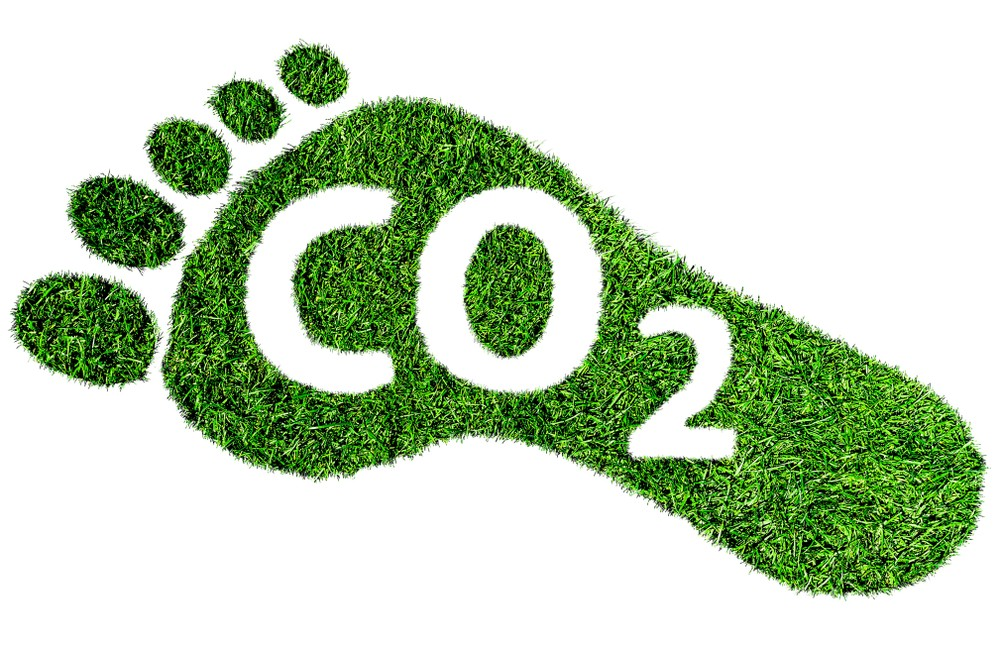
\includegraphics[width=0.3\linewidth]{co2.jpg}
\end{figure}

\pause
\begin{itemize}
\item \textbf{Contribution}: This study systematically compares four models, namely the GHG Protocol, Life-Cycle Assessment, Environmentally Extended Input-Output Analysis, and general equilibrium model of Hakenes–Schliephake to assess attribution differences, empirical consequences, and policy alignment.
\end{itemize}
\end{frame}



% -------------------
\begin{frame}{Research Questions}
\begin{enumerate}
  \item How do footprint estimates vary across models?
 \pause
  \item How is household responsibility estimated and attributed under each carbon accounting method?
  \pause
  \item How do attribution methods shape policy and equity outcomes?
\end{enumerate}
\end{frame}

\begin{frame}{Literature Review: Evolution of HCF Estimation}
\footnotesize
\vspace{-2.5em}
\begin{itemize}
  \item Research on household carbon footprints (HCF) has expanded since the early 2000s, evolving across three broad phases:
  \begin{itemize}
    \footnotesize
    \item \textbf{Early phase:} IO-based estimation of emissions by expenditure category (Pachauri \& Spreng, 2002; Lenzen et. al, 2004)
    \pause
    \item \textbf{Expansion:} 
    \begin{itemize}
    \item Household heterogeneity and national comparisons (Druckman \& Jackson, 2009; Baiocchi \& Minx, 2010)
    \item Integration of inequality and global supply chains (Ivanova et al., 2015; Moran et al., 2018)
    \end{itemize}
  \end{itemize}
\pause
  \item Dominant methods in current literature:
 
  \begin{itemize}
    \pause
    \item  \footnotesize \textbf{Carbon emission coefficient:} Inventory based emission assignment (GHG Protocol under IPCC Guidelines, 2019)
    \pause
    \item \footnotesize \textbf{Life Cycle Assessment:} Process-based alternative, tracing cradle-to-grave emissions (Steubing et al., 2022)
    \pause 
    \item \footnotesize \textbf{Input–Output Analysis:} Economy-wide linkages via input–output matrices (Baiocchi \& Minx; 2010, Wiedmann, 2009)
  \end{itemize}
\end{itemize}
\end{frame}


\begin{frame}{Literature Review: Publication Trends and Focus Areas}
\small
\vspace{-2.5em}
\begin{itemize}
  \footnotesize
  \item A bibliometric analysis of \textbf{1,311 peer-reviewed articles (2000–2025)} shows a sharp rise post-2015 (Paris Agreement).
  \pause
  \item Research is concentrated around \textit{input–output analysis, sustainable consumption}, and \textit{life cycle assessment}.
  \end{itemize}
\vspace{-1.0em}
\begin{columns}
  \centering
  \begin{column}{0.5\textwidth}
    \centering
    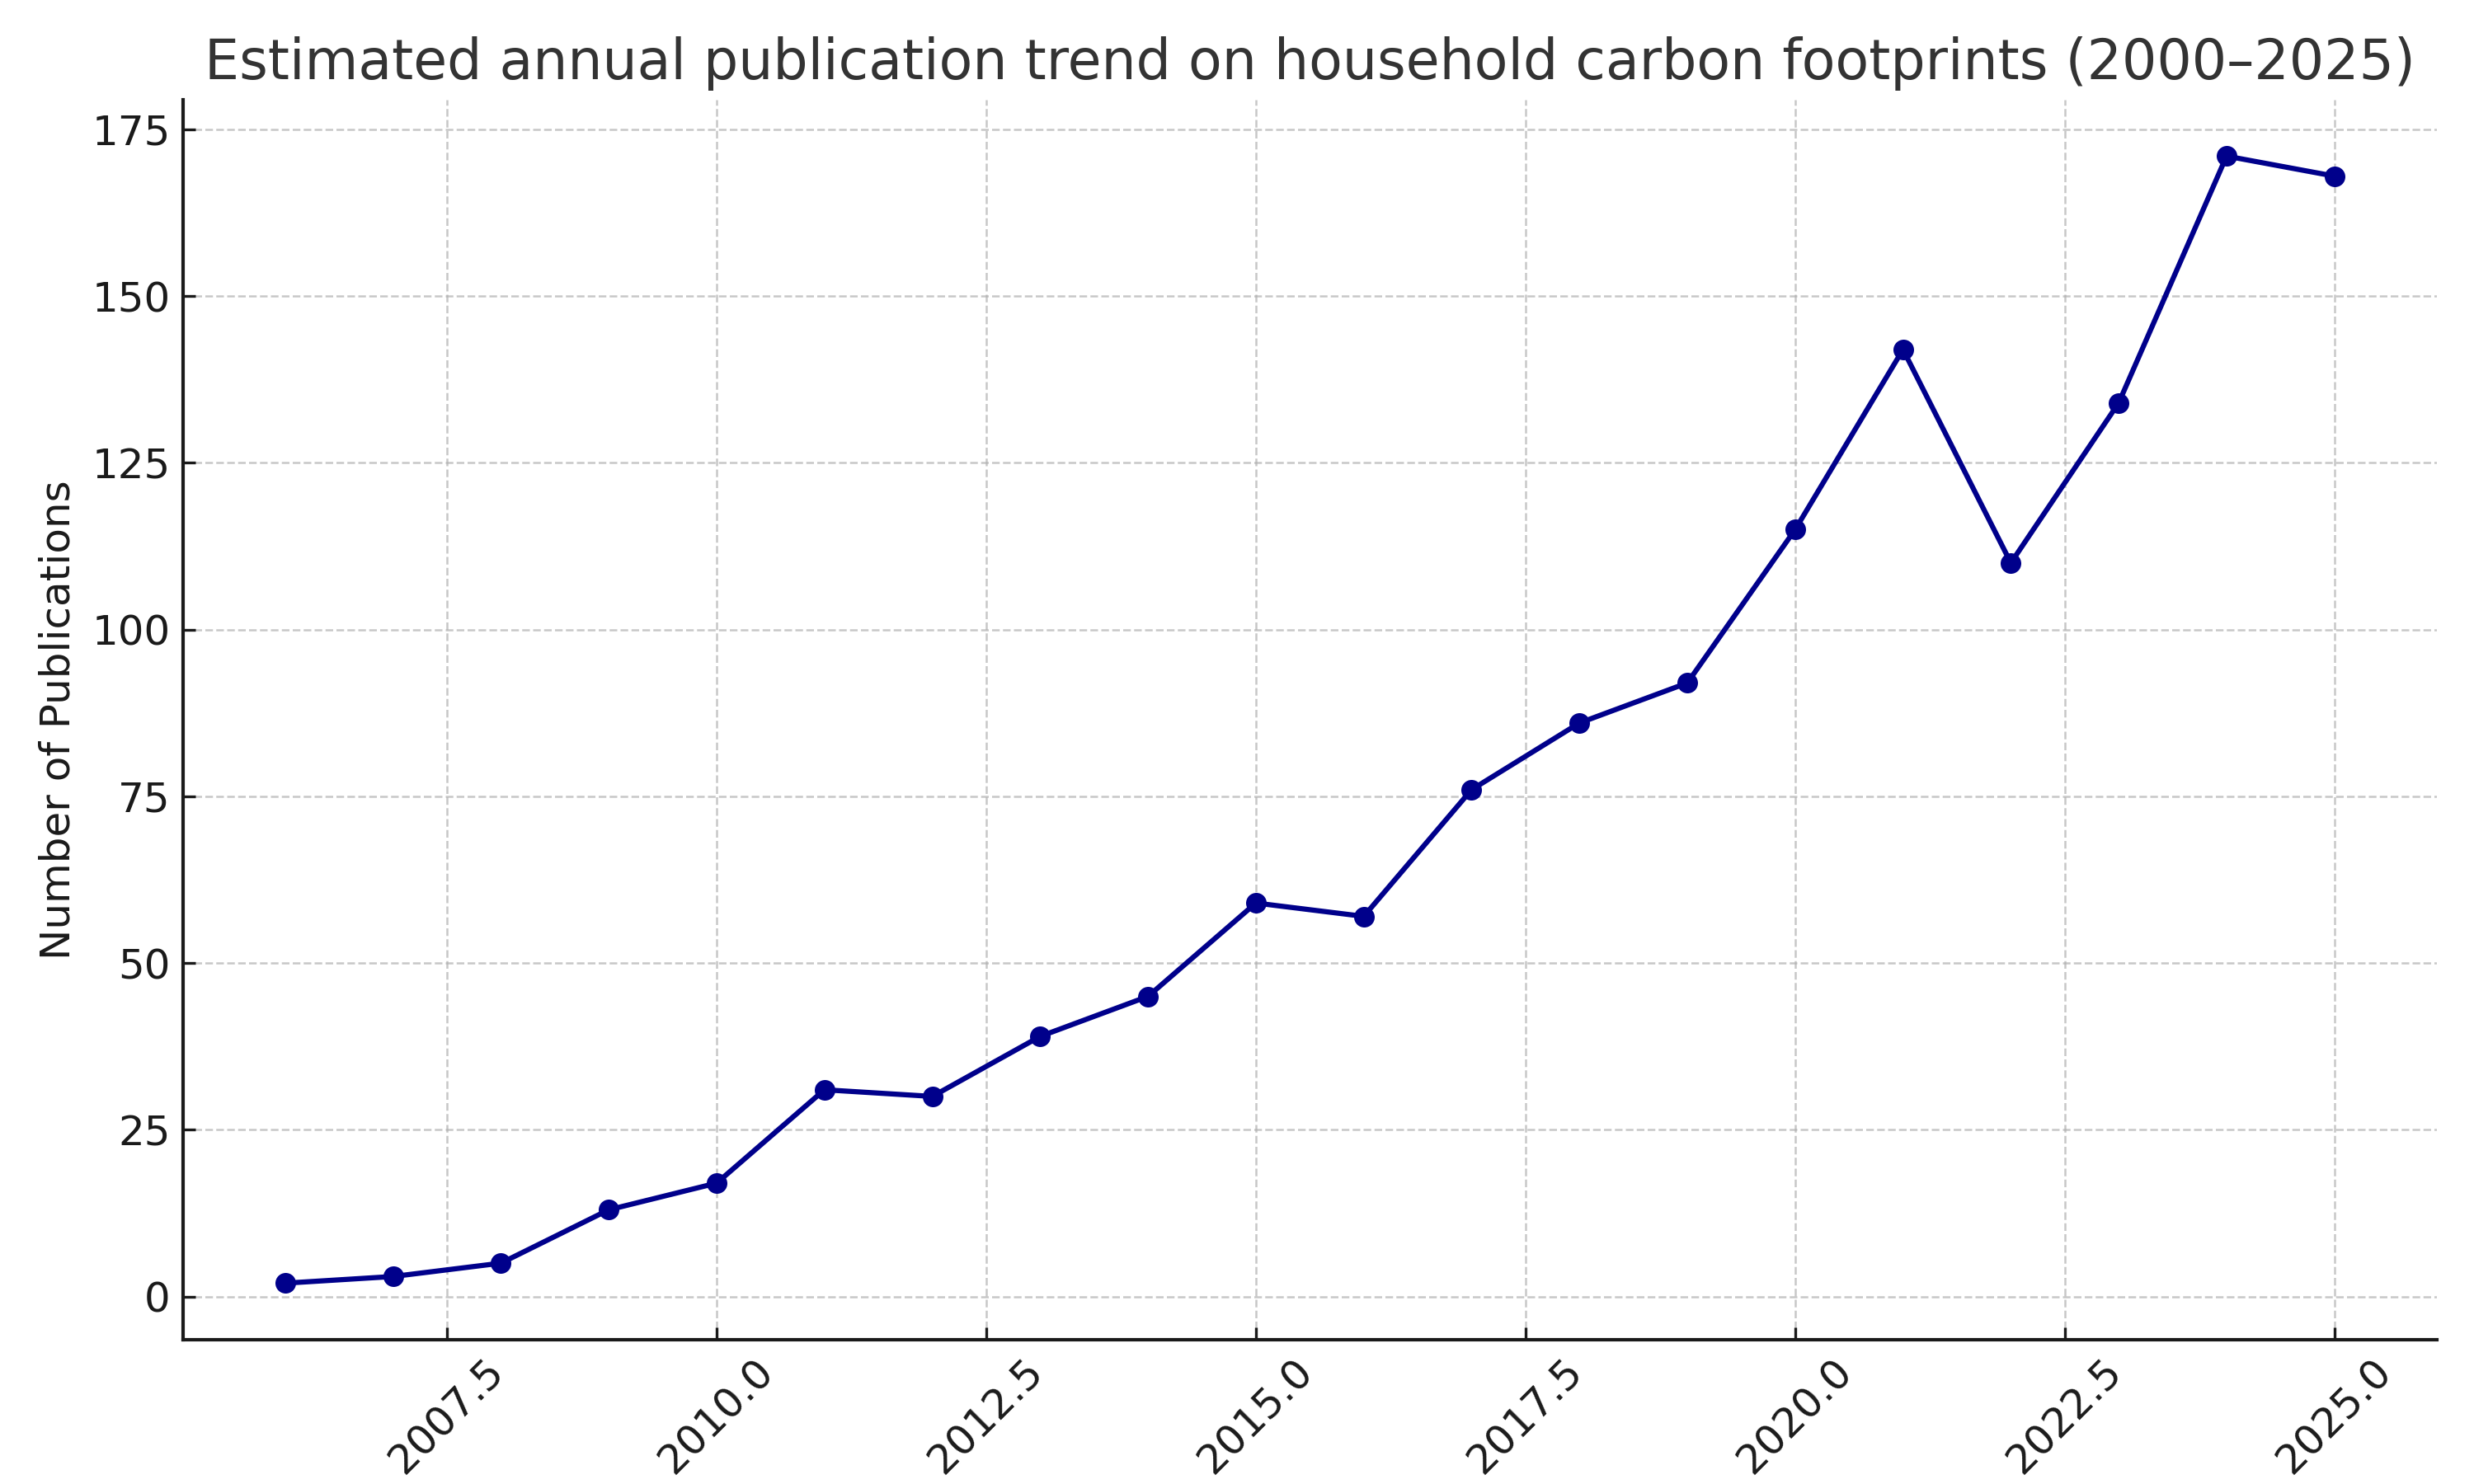
\includegraphics[width=0.8\linewidth]{publication_trend_darkblue_estimated2025.png}
  \end{column}
  \begin{column}{0.6\textwidth}
    \centering
    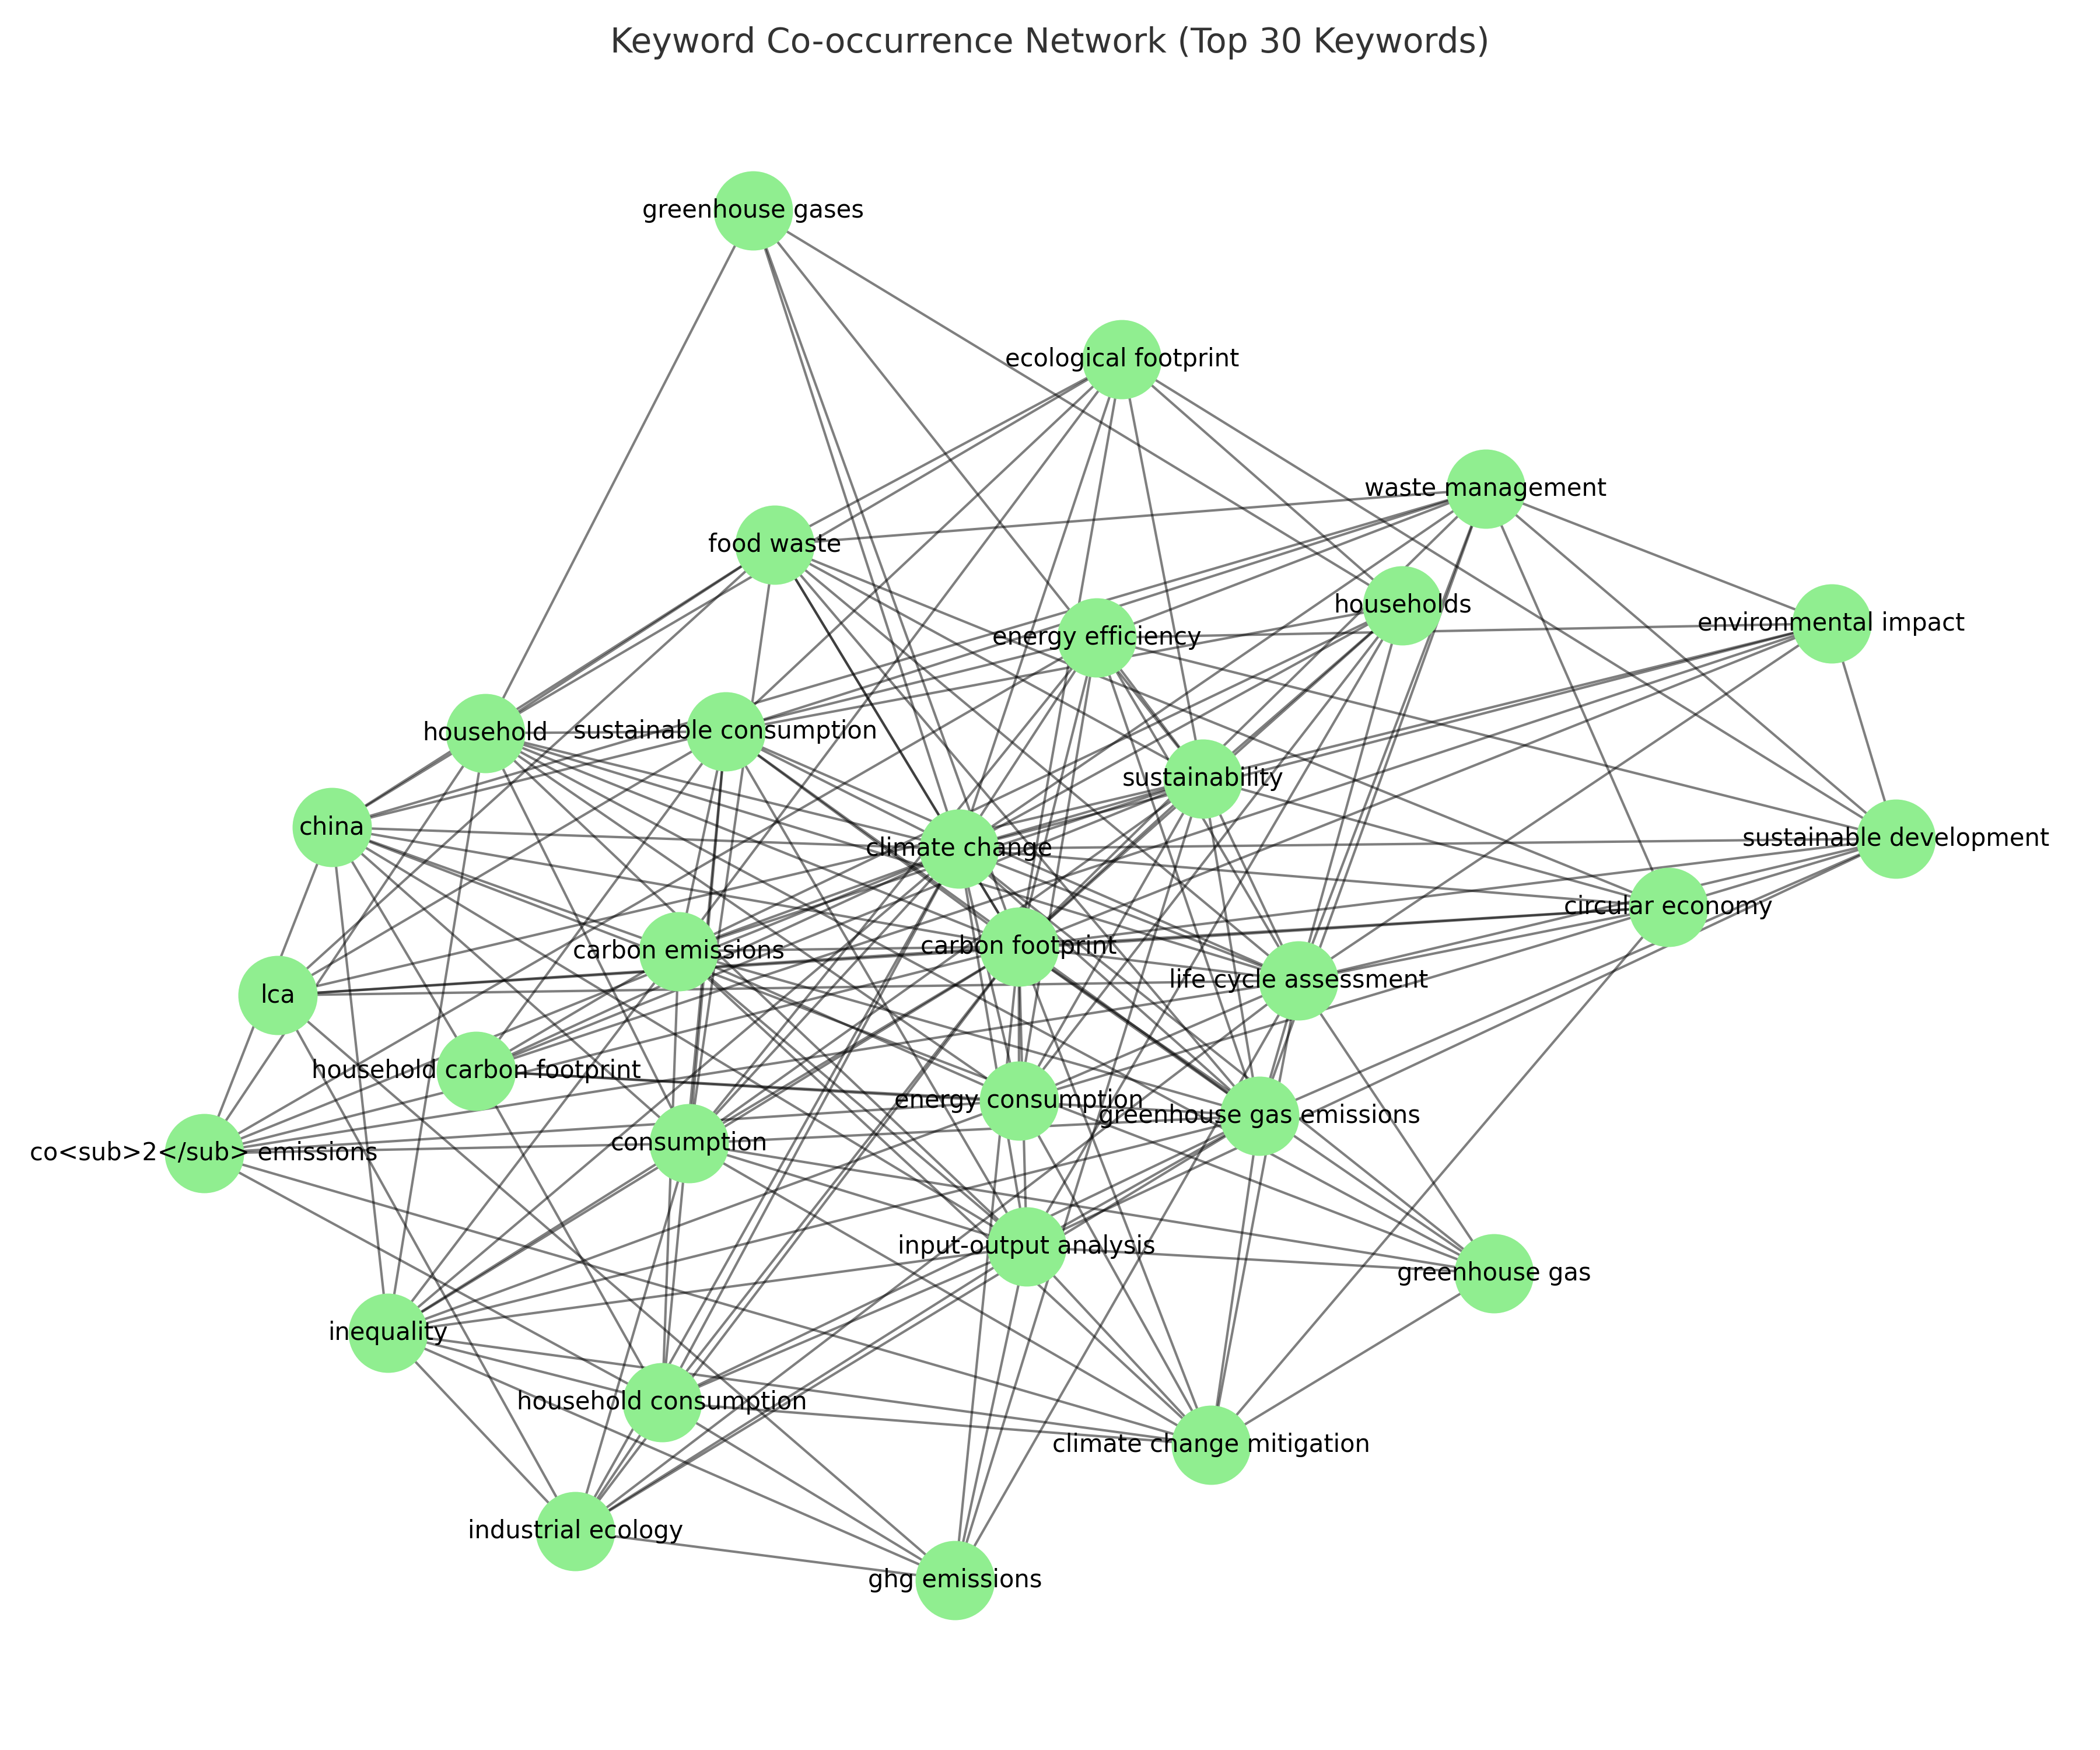
\includegraphics[width=0.7\linewidth]{keyword_cooccurrence.png}
  \end{column}
\end{columns}
\pause
\vspace{-0.5em}
\begin{itemize}
  \footnotesize
\item Top Journals: \textit{Journal of Cleaner Production}, \textit{Science of the Total Environment}, and \textit{Environmental Science \& Technology}
  \item Top institutions: University of Tokyo, Sun Yat-sen University, University of Maryland.
\end{itemize}

\end{frame}


\begin{frame}{Methodology}
\footnotesize
\vspace{-2.5em}
\begin{itemize}
\item A comparative framework is used to analyze how different carbon accounting methods estimate and attribute household emissions.
\pause
\item Models are derived and illustrated using official household expenditure data (Eurostat, USDA) and publicly available emission factors (EXIOBASE, Climatiq, IPCC, DEFRA).
\pause
\item Each model is classified an attribution logic as operational, consumption-based, or consequentialist based on its scope.
\pause
\item Each attribution model is linked to relevant policy instruments and their distributional impacts.
\end{itemize}
\pause
\begin{figure}
\centering
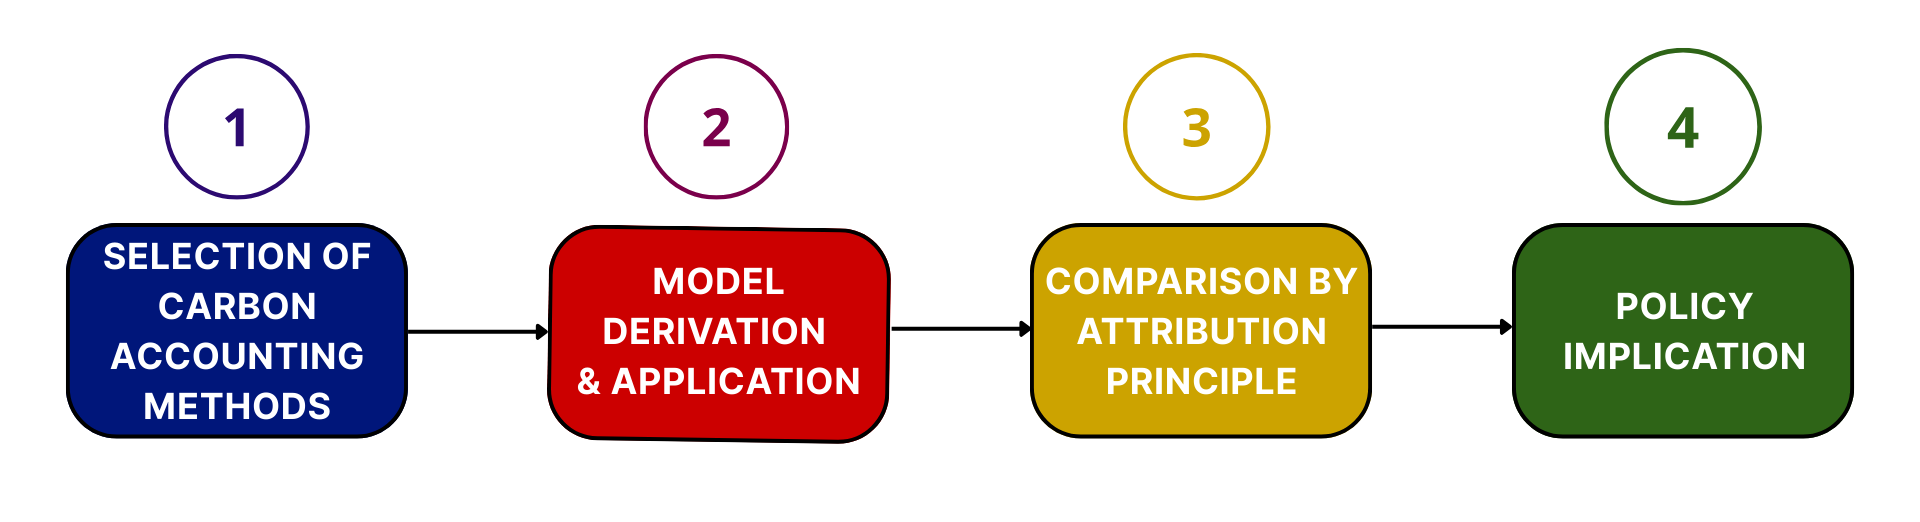
\includegraphics[width=\linewidth]{Methodology chart.png}
\end{figure}
\end{frame}

%create a flowchart for comparison basis: Derivation->Estimation->Attribution->Policy Implications

\begin{frame}{The GHG Protocol}
\small
\vspace{-2.5em}

\footnotesize \textbf{Definition:}  
The Greenhouse Gas (GHG) Protocol is a standardized framework developed by WRI and WBCSD for tracking emissions across three scopes.
\vspace{-0.5em}
\pause
\begin{figure}[h]
  \centering
  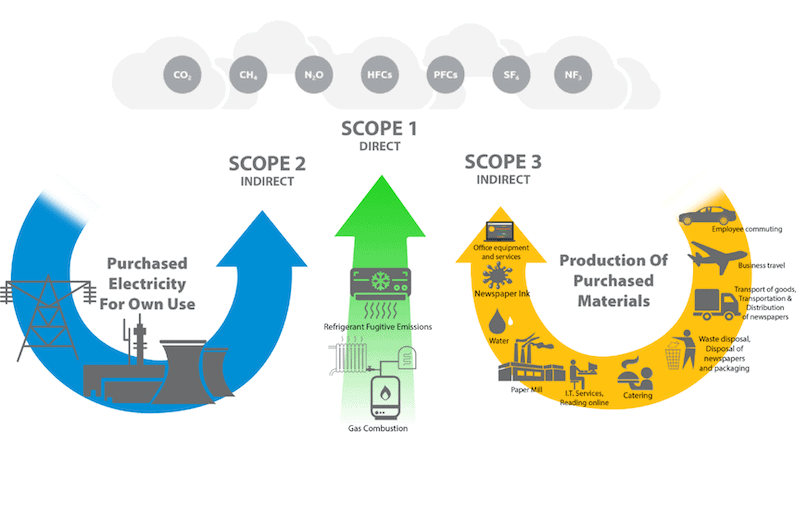
\includegraphics[width=0.55\linewidth]{ghg scope.png}
  \caption*{\tiny Source: Green Element (2023) — https://greenelement.co.uk}
\end{figure}
\vspace{-1.0em}
\pause
\footnotesize \textbf{Formulation:}
\[
\text{CF}_{\text{household}} = E_{\text{Scope 1}} + E_{\text{Scope 2}} + E_{\text{Scope 3}}, \quad 
E_i = \sum_j Q_{ij} \cdot EF_{ij}
\]
{\footnotesize where $Q_{ij}$ is the activity level and $EF_{ij}$ is the emission factor for activity $j$ under scope $i$.}

\end{frame}

\section{Methods \& Applications}

\begin{frame}{GHG Protocol – Empirical Application (Spain, 2022)}
\vspace{-2.5em}
  \footnotesize
  \begin{itemize}
\item \textbf{Objective:} Estimate average household emissions by scope using GHG Protocol.\\

\pause
\item \textbf{Method: }Scope 1, 2, and 3 emissions are calculated using the GHG Protocol's framework using data on Spanish household expenditure and energy use (INE 2022) and emission factors sourced from DEFRA (2022) and IPCC (2019).\\
  \end{itemize}
\pause
%make this into a pie chart
\vspace{-0.5em}
\begin{figure}
\centering
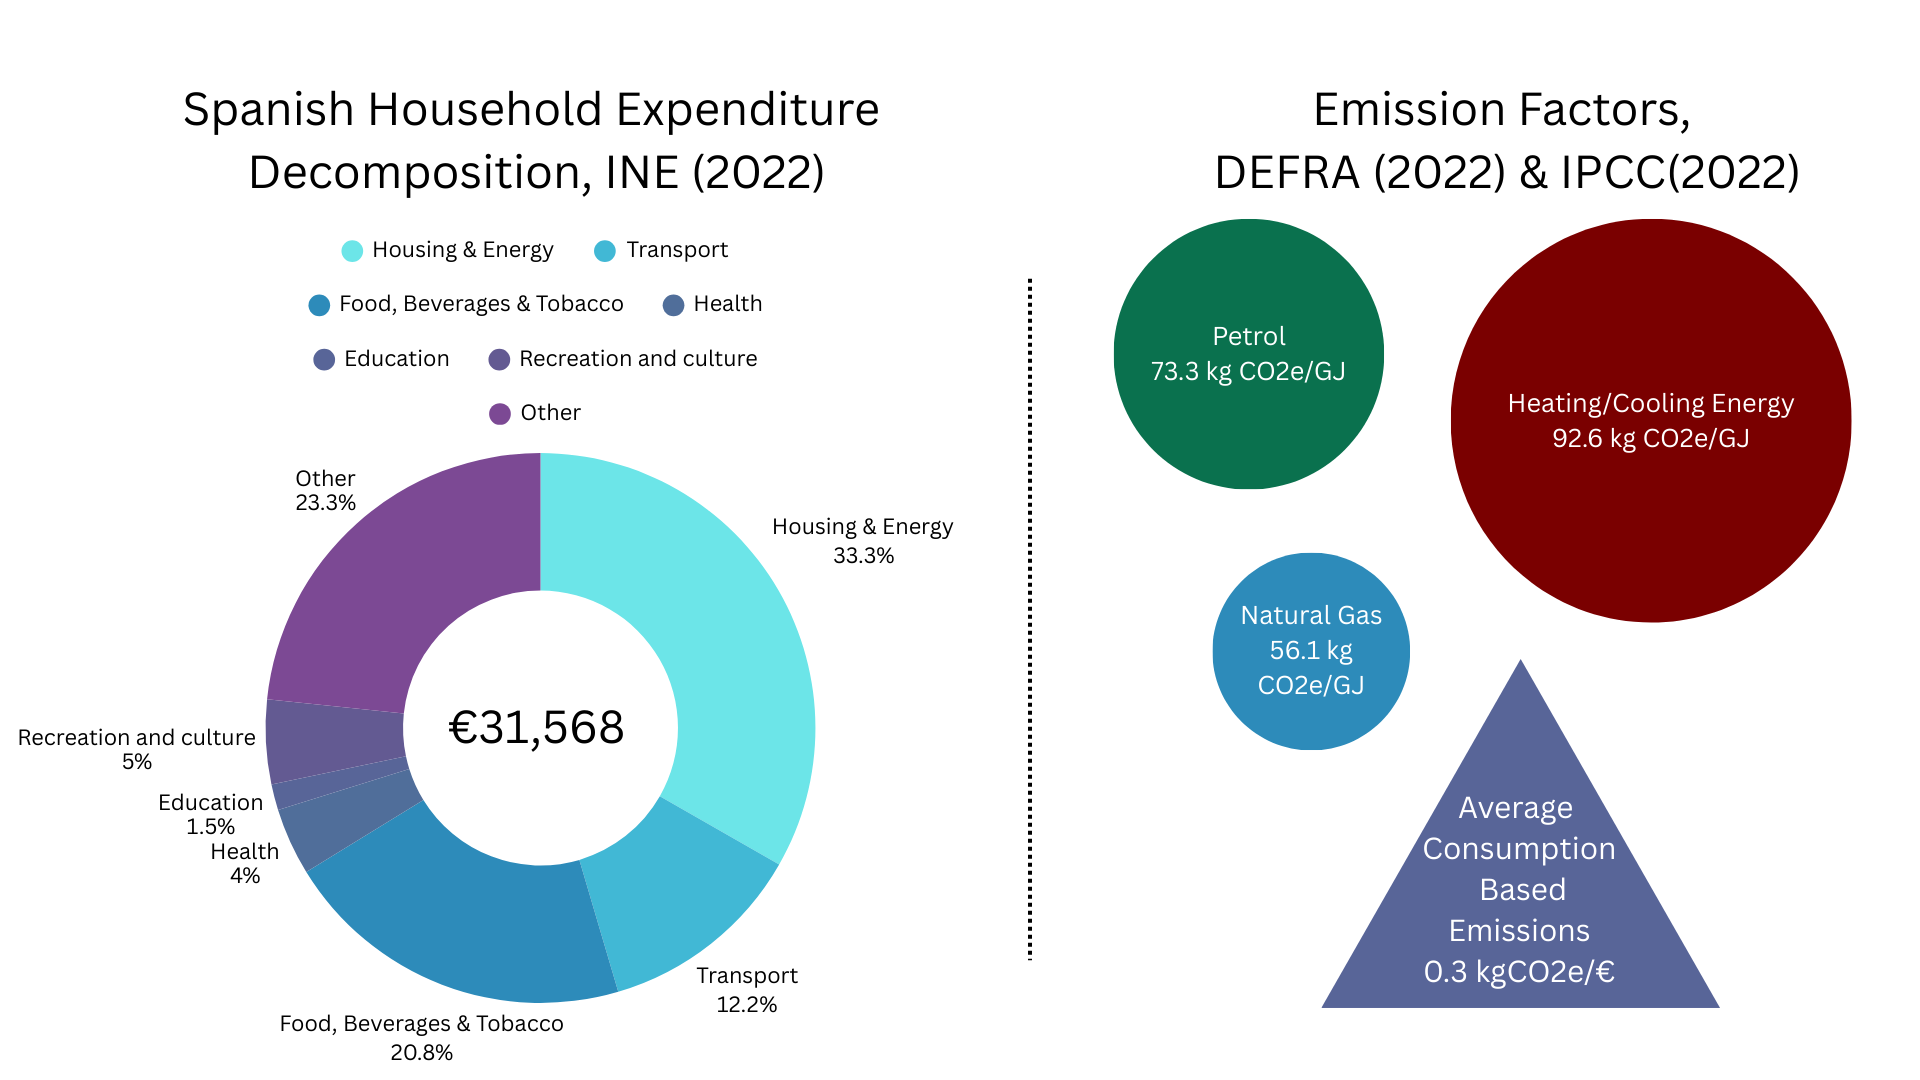
\includegraphics[width=0.8\linewidth]{Spanish Data Visual.png}
\end{figure}



\end{frame}

\begin{frame}{GHG Protocol – Empirical Results (Spain, 2022)}
\vspace{-2.0em}
\footnotesize
\textbf{Total Household Carbon Footprint:}  
\[
\text{Total Emissions} = 11,828.08 \text{ kg CO}_2\text{e/year}
\]
\pause
\vspace{0.5em}
\textbf{Emissions by Scope}
\begin{table}[h!]
\small
\centering
  \resizebox{\textwidth}{!}{%
\begin{tabular}{lccc}
\toprule
\textbf{Scope} & \textbf{Definition} & \textbf{Emissions (kg CO\textsubscript{2}e)} & \textbf{Share (\%)} \\
\midrule
Scope 1 & Direct fuel use (transport + heating) & 1,114.83 & 9.4\% \\
Scope 2 & Purchased electricity/heating & 829.70 & 7.0\% \\
Scope 3 & Lifecycle emissions from consumption & 9,883.55 & 83.6\% \\
\midrule
\textbf{Total} &  & \textbf{11,828.08} & \textbf{100\%} \\
\bottomrule
\end{tabular}}
\end{table}
\pause
\footnotesize
\textbf{Key Findings}
\begin{itemize}
  \item Over 80\% of emissions stem from scope 3 indirect consumption (e.g., food, housing, services).
  \item Scopes 1 and 2 combined account for less than 20\%.
\end{itemize}

\pause
\vspace{0.5em}
\textbf{Conclusion:}  
The GHG Protocol effectively captures direct emissions but underestimates total responsibility unless Scope 3 is comprehensively integrated.

%include limitations? Remove the previous slide?
\end{frame}

\begin{frame}{Life Cycle Assessment (LCA)}
\footnotesize
\vspace{-2.5em}
\begin{itemize}
\item Life Cycle Assessment (LCA) calculates greenhouse gas emissions across the full life cycle of a product or service, from resource extraction and production to use and end-of-life disposal assigning life cycle emission factors to household consumption in units using the \textbf{$fp_h = q_h \cdot \text{LCA}_j$} principle. 
\pause
\item This method captures both direct and embodied emissions by integrating three complementary approaches:
\end{itemize}
\vspace{-0.5em}
\begin{figure}
\centering
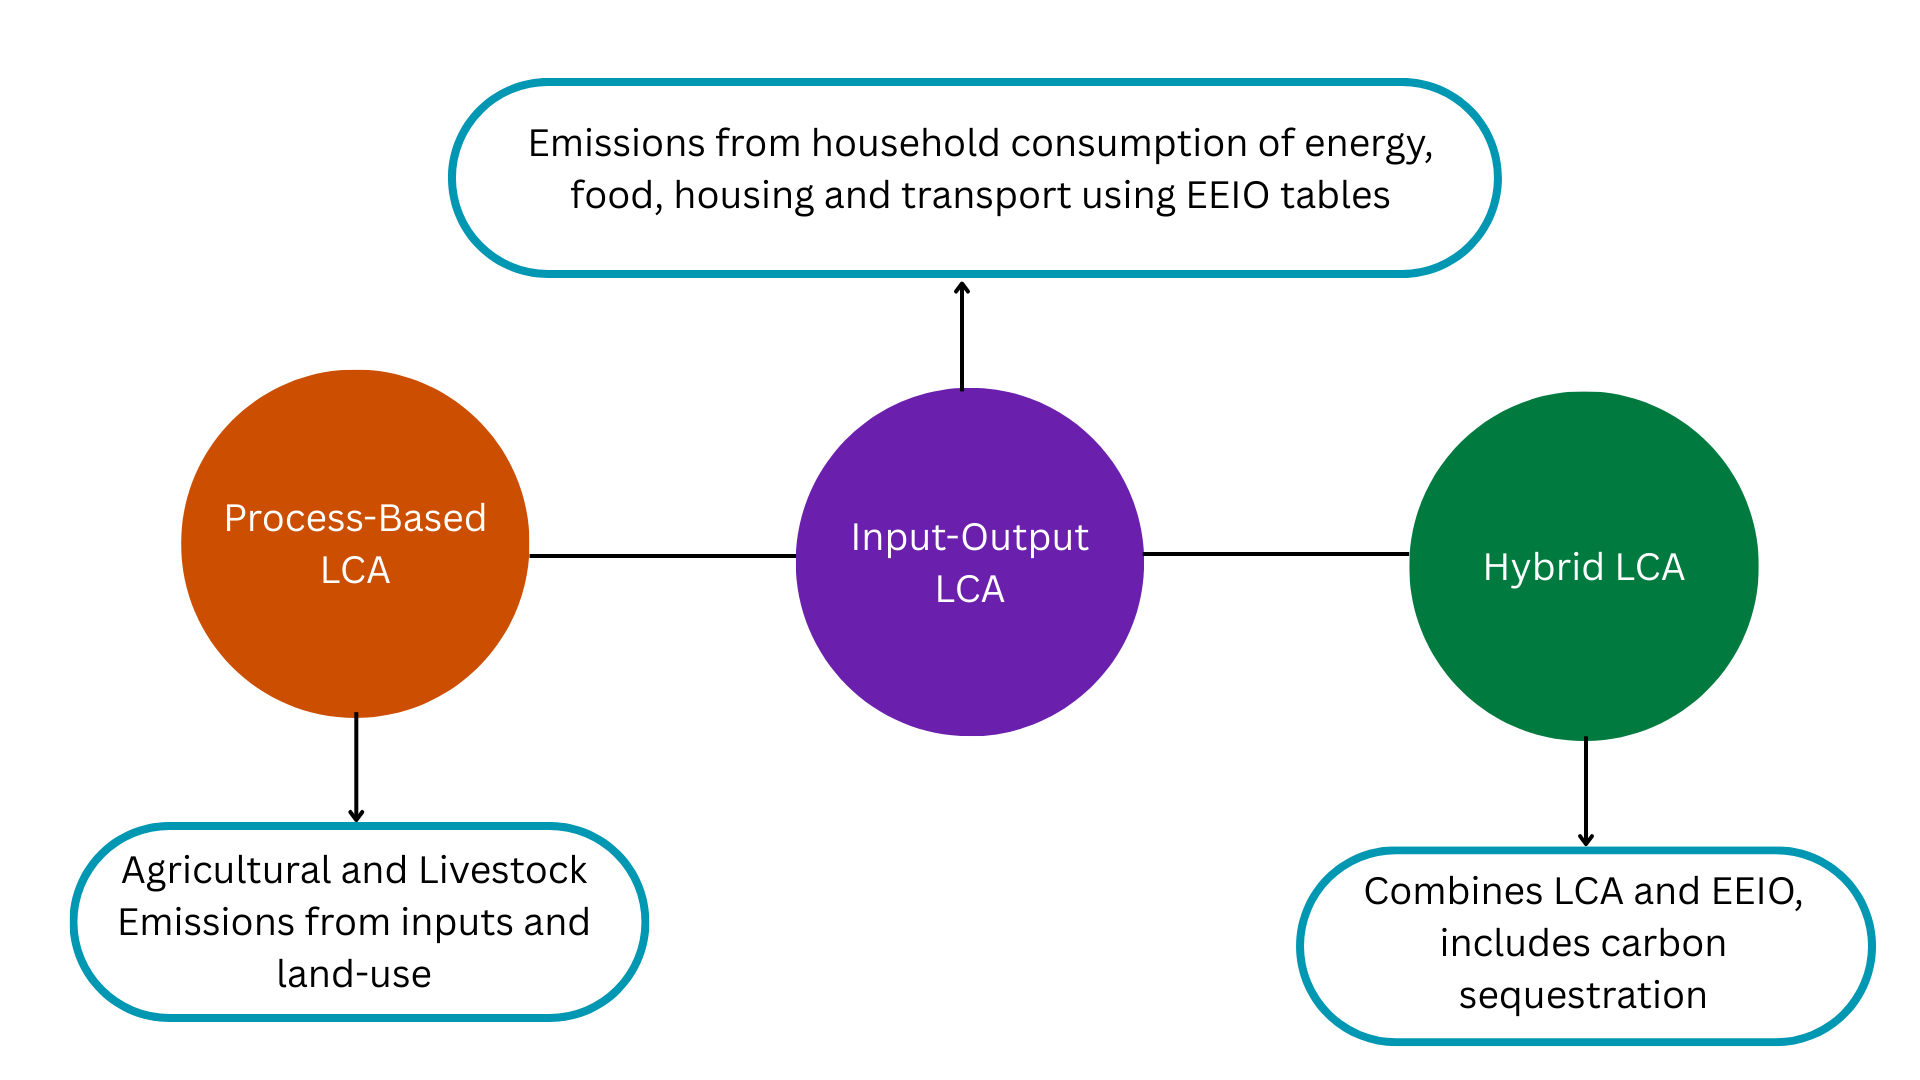
\includegraphics[width=0.7\linewidth]{LCA Visual.png}
\end{figure}
\end{frame}

\begin{frame}{Life Cycle Assessment (LCA): Integrated Estimation}
\footnotesize
\vspace{-2.5em}
\textbf{Framework:}  
Adapted from Peng et al. (2021), the hybrid LCA model aggregates activity-based emissions and sequestration:
\pause
\[
CF_i = \sum_n E_{in} + \sum_m S_{im}
\quad \text{(emissions + sequestration)}
\]
\pause
\vspace{0.3em}
\textbf{Functional Components:}
\begin{itemize}
  \item \textbf{Direct Energy Use:} $E_{id} = \sum_d (F_{id} \cdot EF_d)$
  \pause
  \item \textbf{Consumption:} Short-lived: $E_{if} = \sum_f (EF_f \cdot C_{if})$  
        Durable: $E_{ij} = \sum_j \frac{EF_j \cdot C_{ij}}{L_j}$
  \pause
        \item \textbf{Agriculture:} $CF_{ia} = \sum_a EF_a M_{ia} + \sum_t EF_t FS_{ia} + \sum_v B_v \cdot 0.475$
  \pause
        \item \textbf{Afforestation (Sequestration):} $S_{iaf} = FS_{iaf} \cdot CS_{\text{citrus}}$
  \pause
        \item \textbf{Livestock:} $E_{il} = \sum_f EF_{if} F_{if} + \sum_l EF_{il} N_{il}$
\end{itemize}

\pause
\vspace{0.3em}
\textbf{Implication:}  
The Hybrid LCA structure reduces truncation error and better reflects household-level carbon responsibility particularly in domains such as food, housing, and land use.
\end{frame}

\begin{frame}{Life Cycle Assessment (LCA): Illustration}
\vspace{-2.5em}
\footnotesize
\pause
\begin{itemize}
  \item Indirect emissions from food, goods, and services dominate household carbon footprints highlighting the limits of focusing solely on energy behavior.
\end{itemize}
\pause
\begin{center}
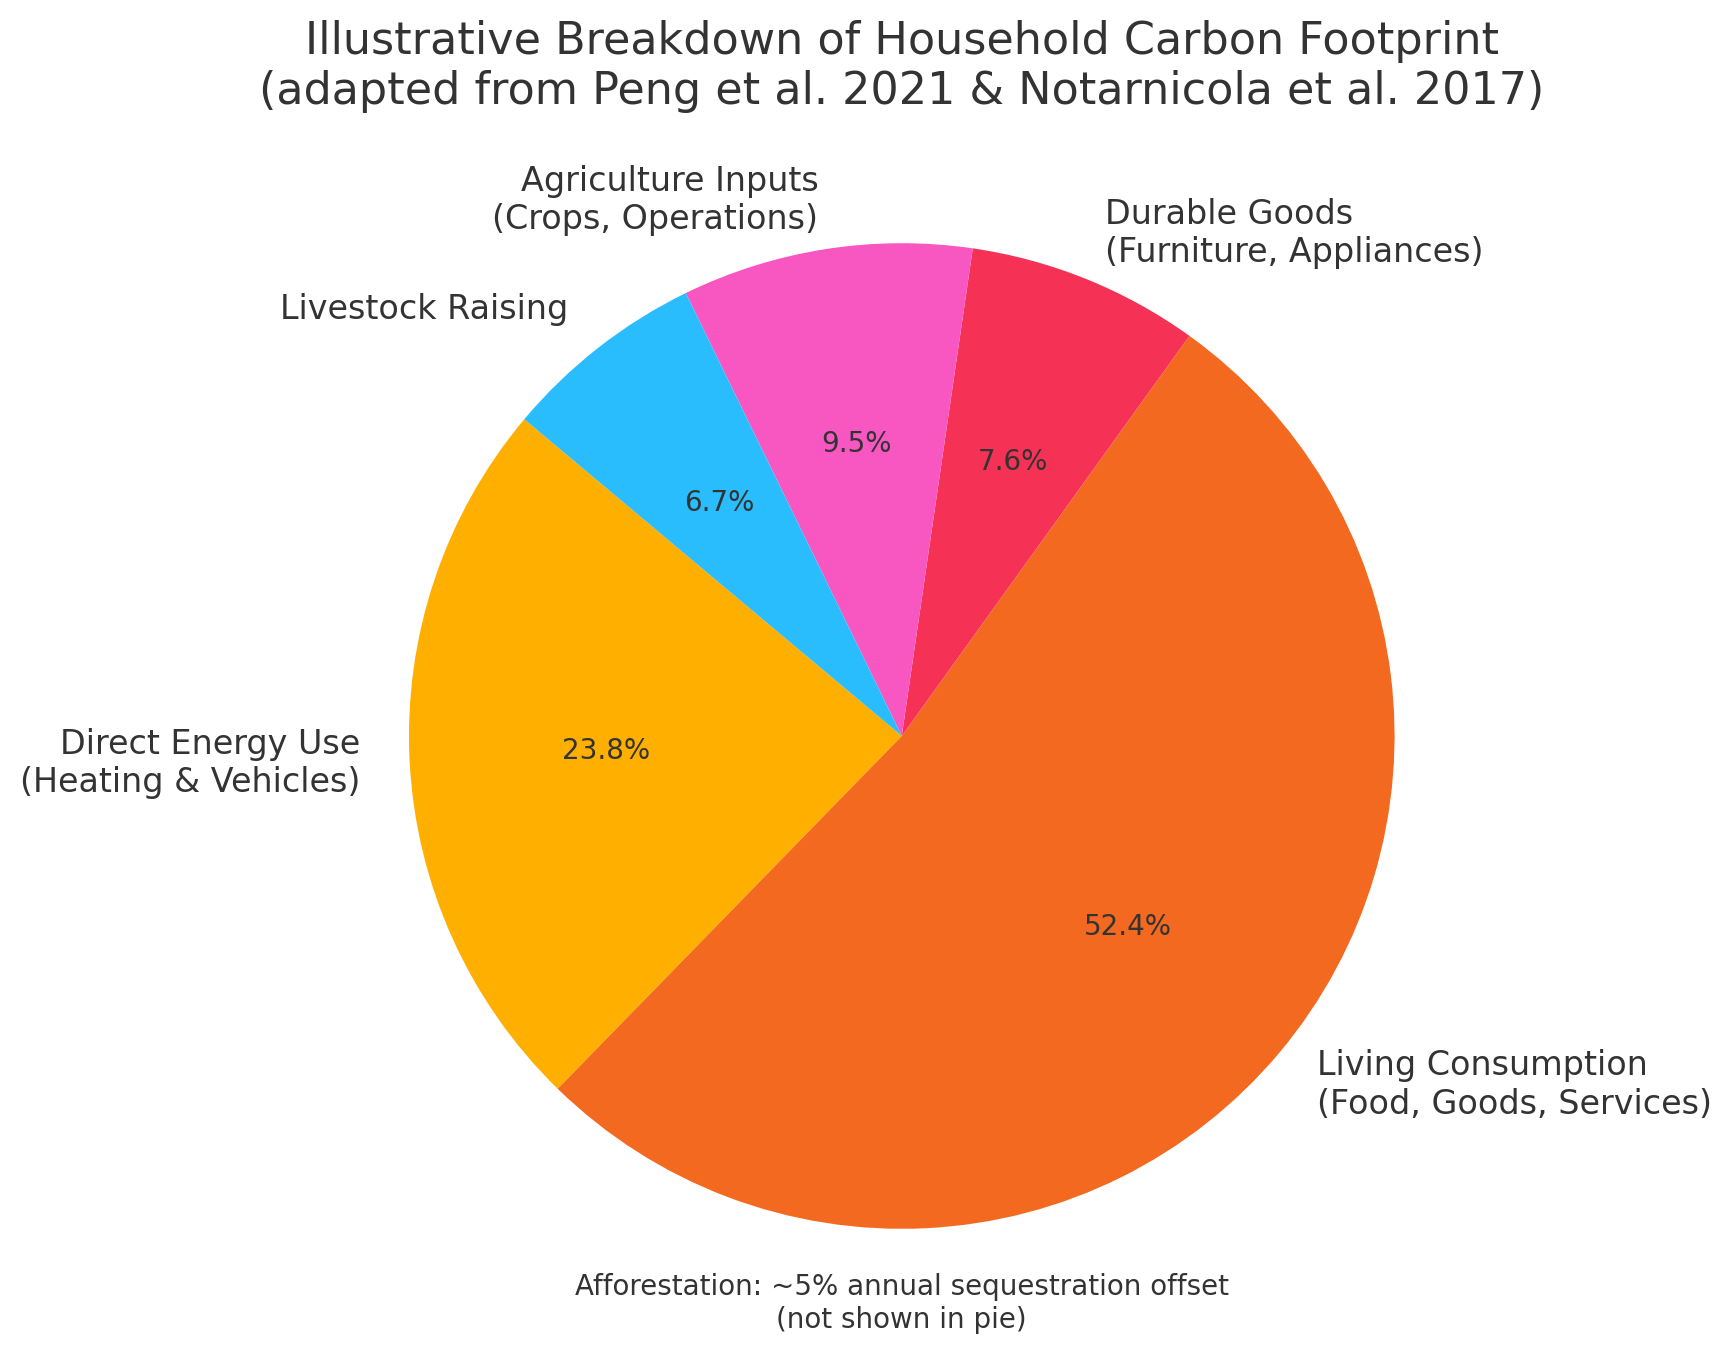
\includegraphics[width=0.68\linewidth]{LCA_pie.png}
\end{center}


\end{frame}

\begin{frame}{Environmentally Extended Input–Output (EEIO) Model}
\footnotesize
\vspace{-2.5em}
\pause
\textbf{Definition:}  
The EEIO model quantifies household carbon footprints by tracing both direct and upstream emissions embedded in goods and services using macroeconomic inter-industry linkages.\\
\pause
\vspace{0.5em}
\textbf{Core Identity:}
\[
\mathbf{X} = (\mathbf{I} - \mathbf{A})^{-1} \cdot \mathbf{F}
\quad
\Rightarrow
\quad
\mathbf{E} = \mathbf{C} \cdot (\mathbf{I} - \mathbf{A})^{-1} \cdot \mathbf{F}
\]

\vspace{0.5em}
\textbf{Components:}
\begin{itemize}
  \item \( \mathbf{A} \): Technical coefficient matrix gives the economic input structure
  \item \( \mathbf{F} \): Final demand vector captures household expenditure
  \item \( \mathbf{C} \): Emission intensity vector (kg CO\textsubscript{2}e / € output)
\end{itemize}

\vspace{0.5em}
\vspace{0.5em}
\pause
\textbf{Model Assumptions and Stability:}
\begin{itemize}
  \item Fixed production coefficients (Leontief structure)
  \item No substitution across sectors or inputs
  \item The matrix \( \mathbf{A} \) must satisfy \( \rho(\mathbf{A}) < 1 \) for stability
  \item Empirically: \( \sum_i A_{ij} < 1 \) for all \( j \)
\end{itemize}

\end{frame}

\begin{frame}{EEIO Emissions Decomposition: Tiered Attribution}
\footnotesize
\vspace{-2.0em}
\pause
Following Matthews et al. (2008) and Long et al. (2019), household emissions are decomposed into three analytical tiers:\\
\pause
\vspace{0.5em}
\textbf{Tier 1 – Direct Emissions:}
\[
\mathbf{E}_1 = \mathbf{C}_d \cdot \mathbf{F}_d
\quad \text{(e.g., direct fuel use)}
\]
\pause
\textbf{Tier 2 – Indirect Energy:}
\[
\mathbf{E}_2 = \mathbf{C}_e \cdot (\mathbf{I} - \mathbf{A})^{-1} \cdot \mathbf{F}_e
\quad \text{(e.g., electricity, heating)}
\]
\pause
\textbf{Tier 3 – Indirect Supply Chain:}
\[
\mathbf{E}_3 = \mathbf{C} \cdot \left[(\mathbf{I} - \mathbf{M})(\mathbf{I} - \mathbf{A})\right]^{-1} \cdot \left[(\mathbf{I} - \mathbf{M}) \cdot \mathbf{F} + \mathbf{EX}\right]
\]
\pause
\vspace{0.5em}
\textbf{Total Household Carbon Footprint:}
\[
\mathbf{E}_{\text{total}} = \mathbf{E}_1 + \mathbf{E}_2 + \mathbf{E}_3
\]
\pause
\vspace{0.5em}
\textbf{Note:}  
Import-adjusted tiers ensure that emissions are attributed to domestic demand. Enables national-scale footprint analysis with high coverage.

\end{frame}

\begin{frame}{EEIO Illustration: Method and Aggregate Estimates}
\vspace{-2.0em} % Adjust vertical space if needed
\footnotesize

\begin{columns}[T] % Align columns at the top
  % Left column: text
  \begin{column}{0.40\textwidth}
    \vspace{2.0em}
    \pause
    \textbf{Methodology:}
    \begin{itemize}
      \item Emission intensities \(EF_i\) reflect \( \mathbf{C}(\mathbf{I}-\mathbf{A})^{-1} \) and are sourced from EXIOBASE (via Climatiq.io).
      \pause
      \item National consumption data on households \(F_{i,c}\) are sourced from Eurostat (2021) for France, Spain and Germany and is multiplied by category-specific \(EF_i\) for each country:
      \[
      E_{i,c} = F_{i,c} \cdot EF_i
      \]
    \end{itemize}
    
    
  \end{column}
\pause
  % Right column: figure
  \begin{column}{0.60\textwidth}
    \centering
    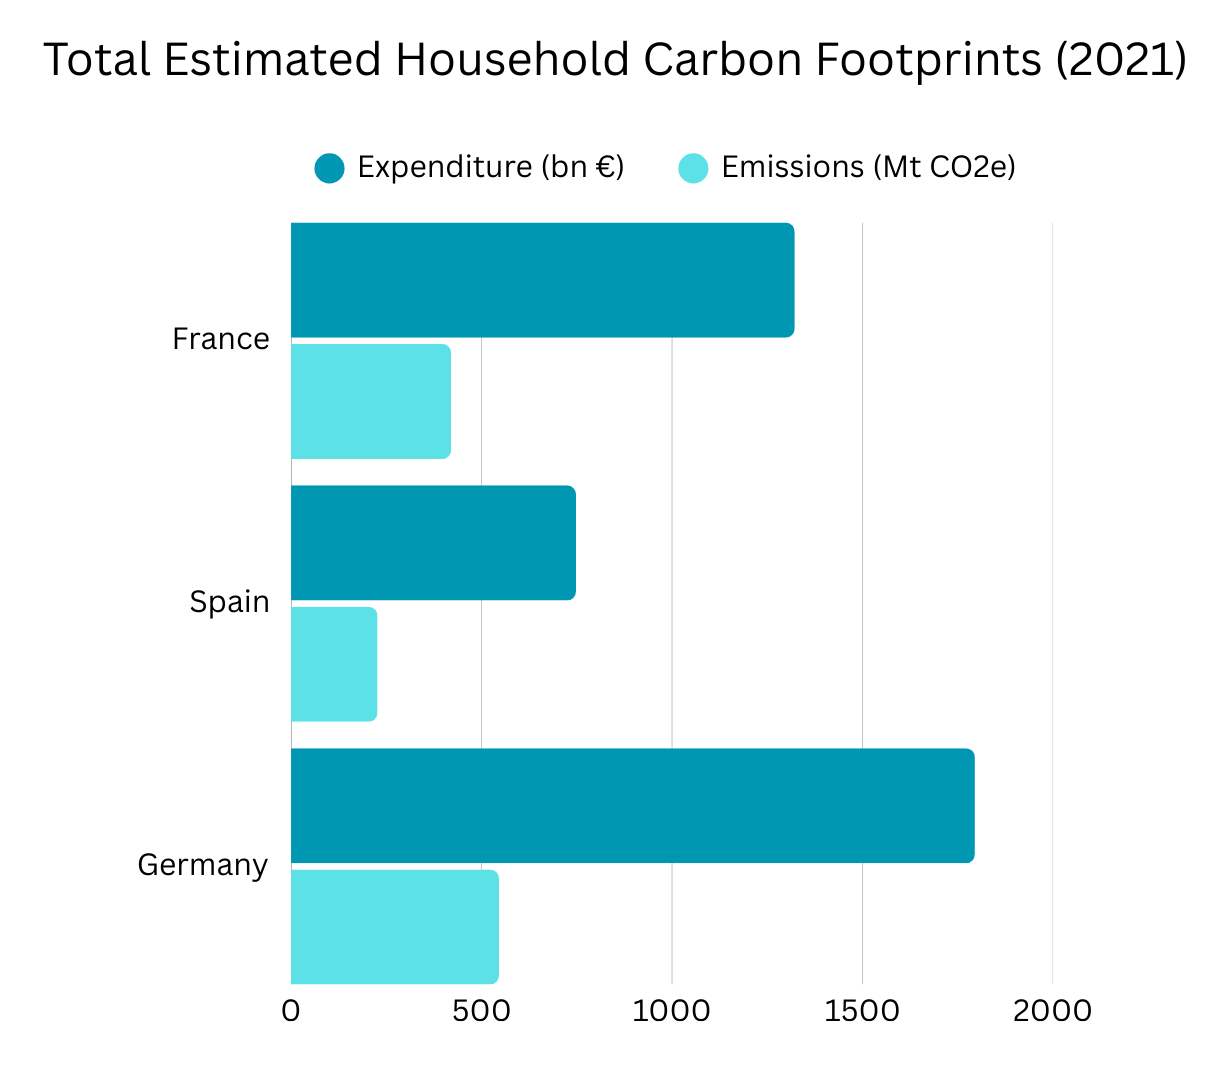
\includegraphics[width=\linewidth]{EEIO Visual.png}

    \footnotesize Source: Eurostat (2021), EXIOBASE (2025); Author’s calculations.
  \end{column}
\end{columns}

\end{frame}



\begin{frame}{EEIO Illustration: Interpretation of Results}
\footnotesize
\vspace{-2.5em}
\textbf{Sectoral Composition of Emissions and Cross-Country Comparison:}
\pause
\begin{figure}
  \centering
  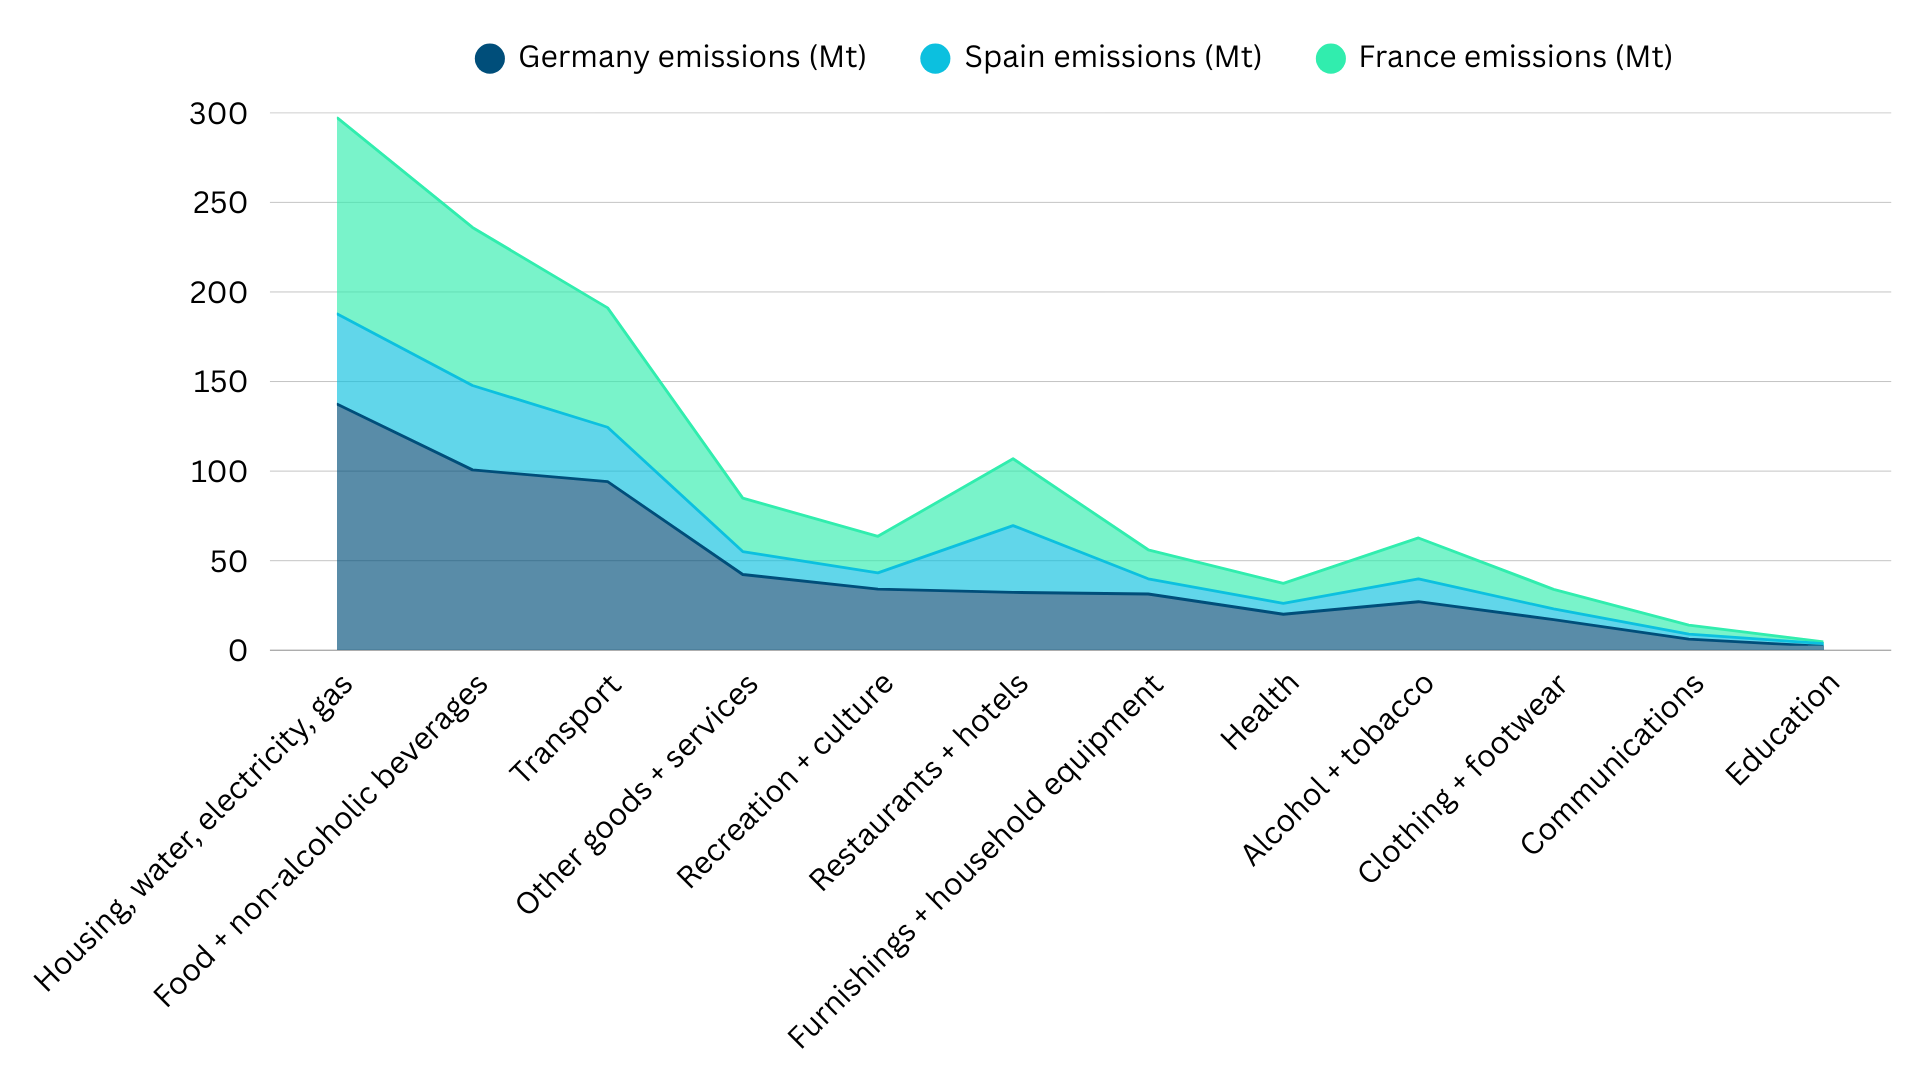
\includegraphics[width=\linewidth]{Emissions EEIO.png}
\end{figure}
\end{frame}

%------------------------------------------------
\begin{frame}{The Hakenes \& Schliephake Model}
\footnotesize
\vspace{-2.5em}
\begin{itemize}
\item Closed general equilibrium model that allocates total footprint of an industry to investment or consumption with industry-specific weights and risk preferences.

\end{itemize}

\pause
\vspace{0.4em}
\textbf{Model Assumptions under One-Industry Economy:}
\begin{itemize}
  \item One homogeneous good produced with capital only, constant returns to scale.
  \item Linear technology: \( I = c Q \)
  \item Firms raise \(I\) from households, repay with \(r = \frac{P}{c} + \lambda + \varepsilon\), with \(\varepsilon \sim \mathcal{N}(0,\sigma^2)\).
  \item Emissions proportional to output: \( X = x Q \).
\end{itemize}

\pause
\textbf{Households:}
\begin{itemize}
  \item Wealth \(w\) allocated to consumption \(q_h\) and investment \(i_h\), residual in risk-free asset (\(r_f\)): $m_h = r i_h + r_f(w - i_h) - P q_h $.
  
  \item Expected Utility:  
  \[
  \mathbb{E}[U_h] = -\exp\left\{ -\alpha \left[ (a - P)q_h - \frac{b}{2}q_h^2 + r_f w + \left( \frac{P}{c} + \lambda - r_f \right)i_h - \frac{\alpha}{2}\sigma^2 i_h^2 - xQ \right] \right\} 
  \]
\end{itemize}

\pause
\textbf{First-Order Conditions:}
\[
q_h = \frac{a - x - P}{b}, \quad 
i_h = \frac{1}{\alpha\sigma^2}\left(\frac{P}{c} + \lambda - r_f\right)
\]
%These capture optimal consumption and investment given prices, risk, and emissions.
\end{frame}
%------------------------------------------------

\begin{frame}{Market Equilibrium and Footprint Derivation}
\footnotesize
\vspace{-2.5em}
\textbf{Market Clearing:}
\[
Q = q_h + (n-1)q_{-h}, \quad I = i_h + (n-1)i_{-h}, \quad I = c Q
\]

\pause
\vspace{0.3em}
\textbf{Supply Curve:}
\[
P = c(r_f - \lambda) + \frac{c^2\alpha\sigma^2}{n-1} Q
\]

\vspace{0.3em}
\textbf{Demand Curve:}
\[
q_{-h} = \frac{a - x - P}{b} \Rightarrow Q = q_h + (n - 1)\cdot \frac{a - x - P}{b} 
\]

\pause
\vspace{0.3em}
\textbf{Solving Supply \& Demand:}
\[
Q = (n-1)\frac{a - x - c(r_f - \lambda)}{b + c^2\alpha\sigma^2} + \phi q_h + (1-\phi)\frac{i_h}{c}
\]
where:
\[
\phi = \frac{b}{b + c^2\alpha\sigma^2}
\]

\textbf{Total Household Carbon Footprint:}
\[
fp_h = x\left(\phi q_h + (1-\phi)\frac{i_h}{c}\right), \quad \sum_h fp_h = x Q
\]
\end{frame}
%------------------------------------------------

%---------------------------------------------
\begin{frame}{Empirical Illustration: U.S. Wheat Market}
\footnotesize
\vspace{-2.5em}
\textbf{Objective:} Apply the single-industry Hakenes--Schliephake model to quantify the impact of supply shocks on the carbon footprint.\\
\pause
\vspace{0.5em}
\textbf{Data \& Market Setup:}
\begin{itemize}
  \item USDA (2010--2017): production volumes (supply), total domestic use (demand), average farm-gate wheat prices.
  \item FAO/USDA: emission factor of 10.88~kg~CO\textsubscript{2}e per bushel.
\item Simulated a 15.6\% production shock (2016–2017).
\item \textbf{Carbon Footprint Calculation: }$
\text{Emissions} = Q_{\text{eq}} \times 10.88 \text{ kg CO\textsubscript{2}e/bushel}
$

\end{itemize}

\pause
\textbf{Empirical Supply Curve:}
\begin{itemize}
  \item Estimated by OLS: \( P = \beta_0 + \beta_1 Q \).
  \item Demand curve: calibrated linear slope from dataset averages.
  
\end{itemize}
\pause
\textbf{Theoretical Supply Curve:}
\[
P(Q) = c(r_f - \lambda) + \frac{c^2 \alpha \sigma^2}{n - 1} Q
\]
\begin{itemize}
  \item Parameters: \(c = 4\), \(r_f = 0.05\), \(\lambda = 0.01\), \(\alpha = 0.5\), \(\sigma = 0.4\), \(n = 100{,}000\).
  \item Demand curve identical to empirical case.
  %\item Captures optimal household capital allocation under risk.
\end{itemize}
\end{frame}

%---------------------------------------------

\begin{frame}{Carbon Footprint under Empirical \& Theoretical Model}
\footnotesize
\pause
\vspace{-3.0em}
\begin{center}
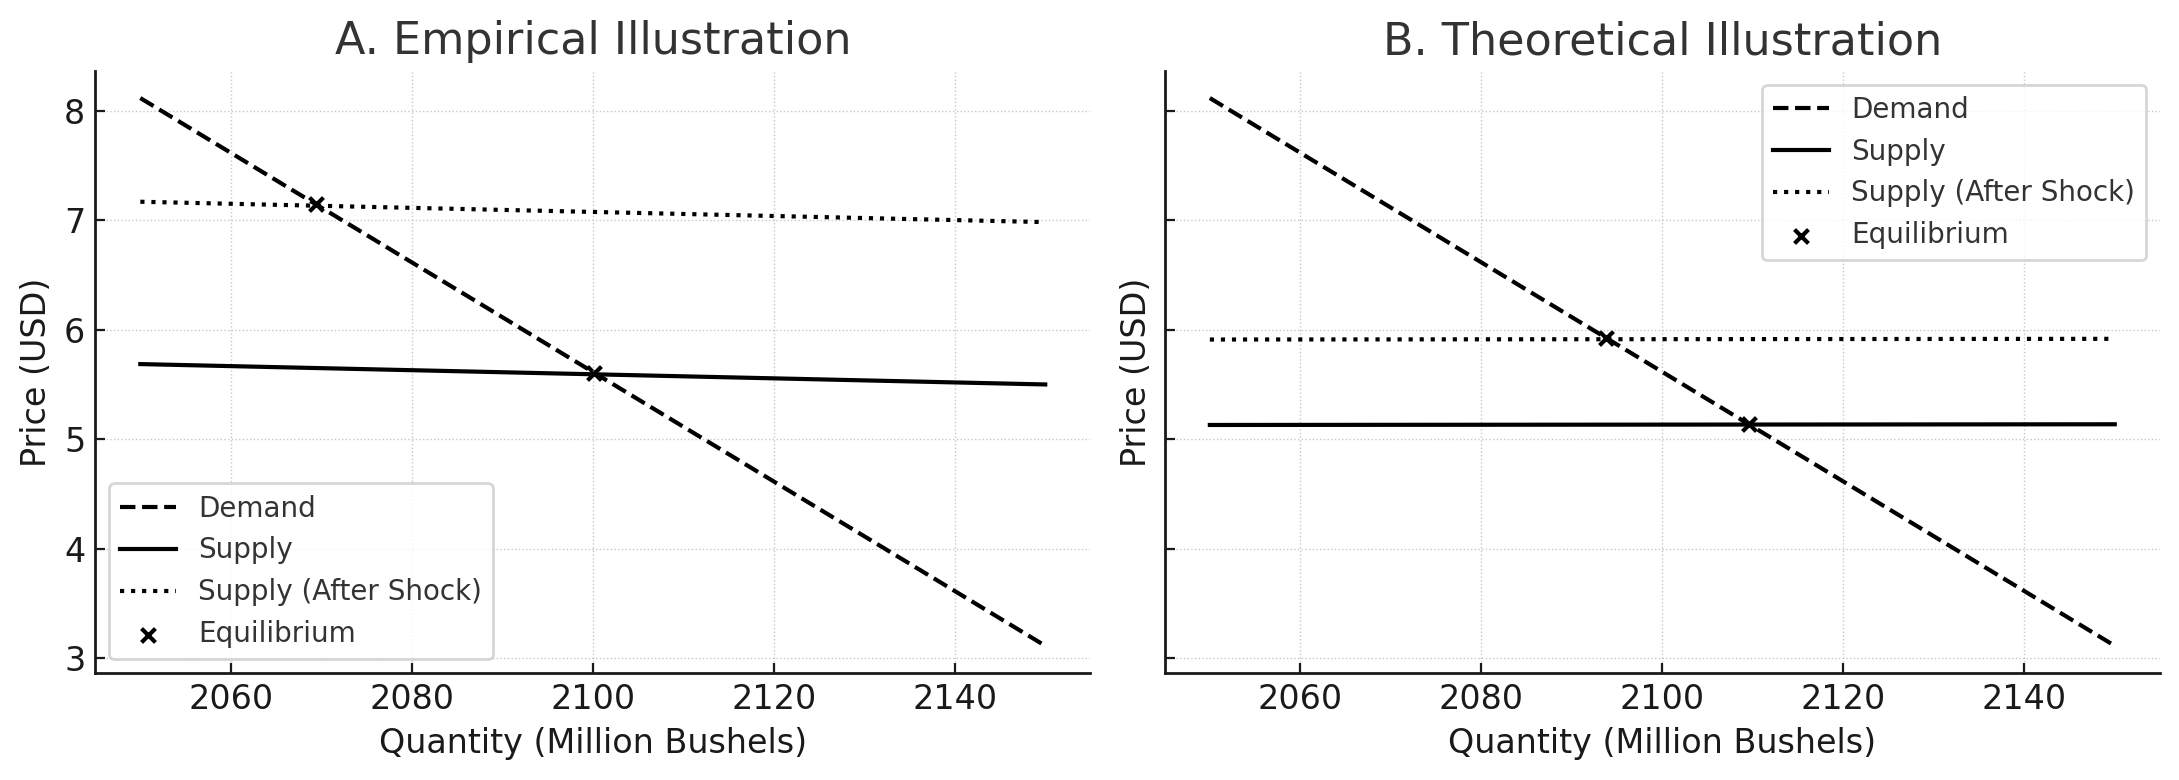
\includegraphics[width=0.9\linewidth]{Hakenes illustration.png}
\end{center}

\pause
\footnotesize
\begin{table}[h!]
\centering
\resizebox{0.8\linewidth}{!}{%
\begin{tabular}{lcc|cc}
\toprule
\textbf{Scenario} & \textbf{Qty (M bu)} & \textbf{CF (M kg CO\textsubscript{2}e)} & \textbf{Qty (M bu)} & \textbf{CF (M kg CO\textsubscript{2}e)} \\
\cmidrule(lr){2-3} \cmidrule(lr){4-5}
 & \multicolumn{2}{c}{\textbf{Empirical Model}} & \multicolumn{2}{c}{\textbf{Theoretical Model}} \\
\midrule
Before  & 2100.71 & 22859.68 & 2112.45 & 22983.46 \\
After   & 2068.38 & 22500.32 & 2096.36 & 22808.40 \\
$\Delta$ & ---     & \textbf{-359.36} & ---     & \textbf{-175.06} \\
\bottomrule
\end{tabular}}
\end{table}


\vspace{0.3em}
\scriptsize Source: Author's calculations based on USDA (2010--2017) and FAO data.


\vspace{0.5em}



\end{frame}


%---------------------------------------------
\section{Responsibility \& Policy Implications}
\begin{frame}{Responsibility for Household Carbon Emissions}
\footnotesize
\vspace{-2.5em}
\textbf{Central Question:}  
How should household responsibility for climate change be defined, measured, and fairly attributed?\\
  \end{frame}


\begin{frame}{Attribution Logics}
  \vspace{-2.5em}
\begin{figure}
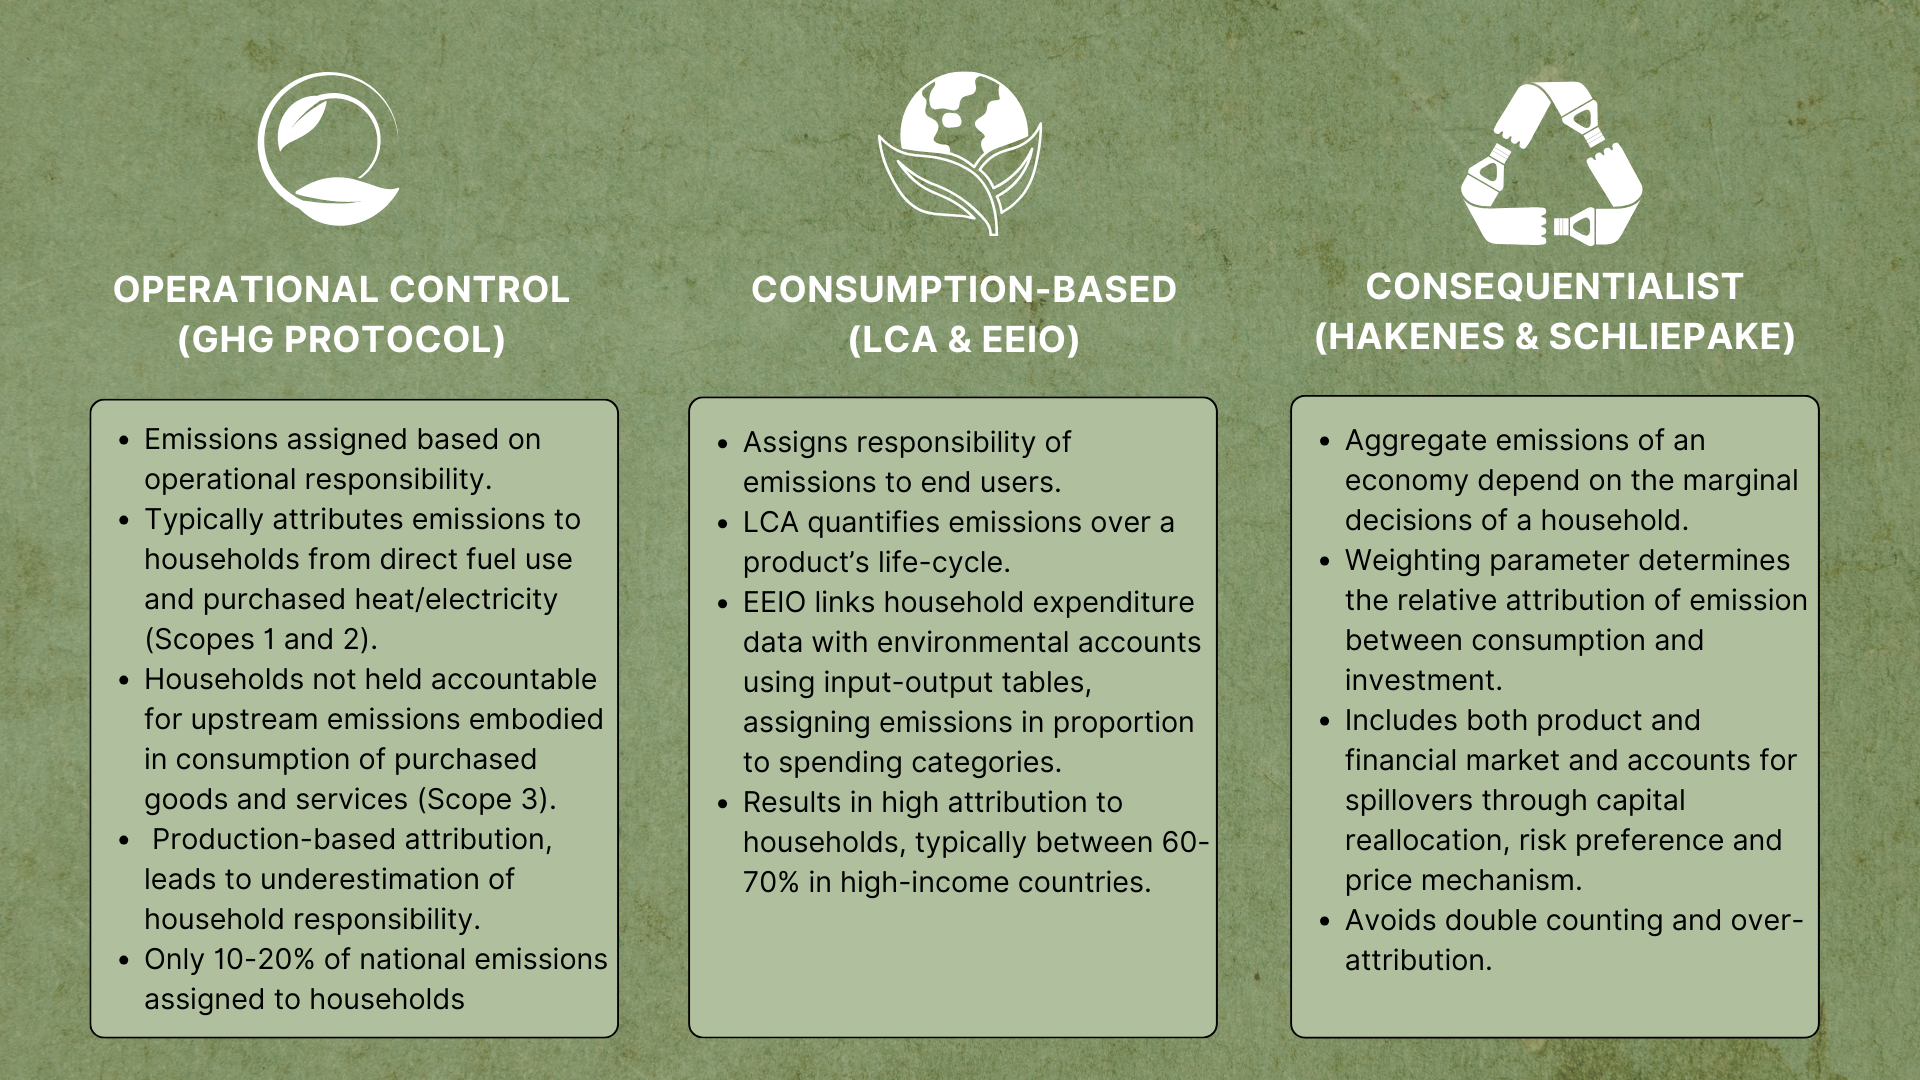
\includegraphics[width=\linewidth]{Operational Control.png}
\end{figure}
\end{frame}

\begin{frame}{Policy Implications of Attribution Logics}
  \vspace{-2.5em}
\begin{figure}
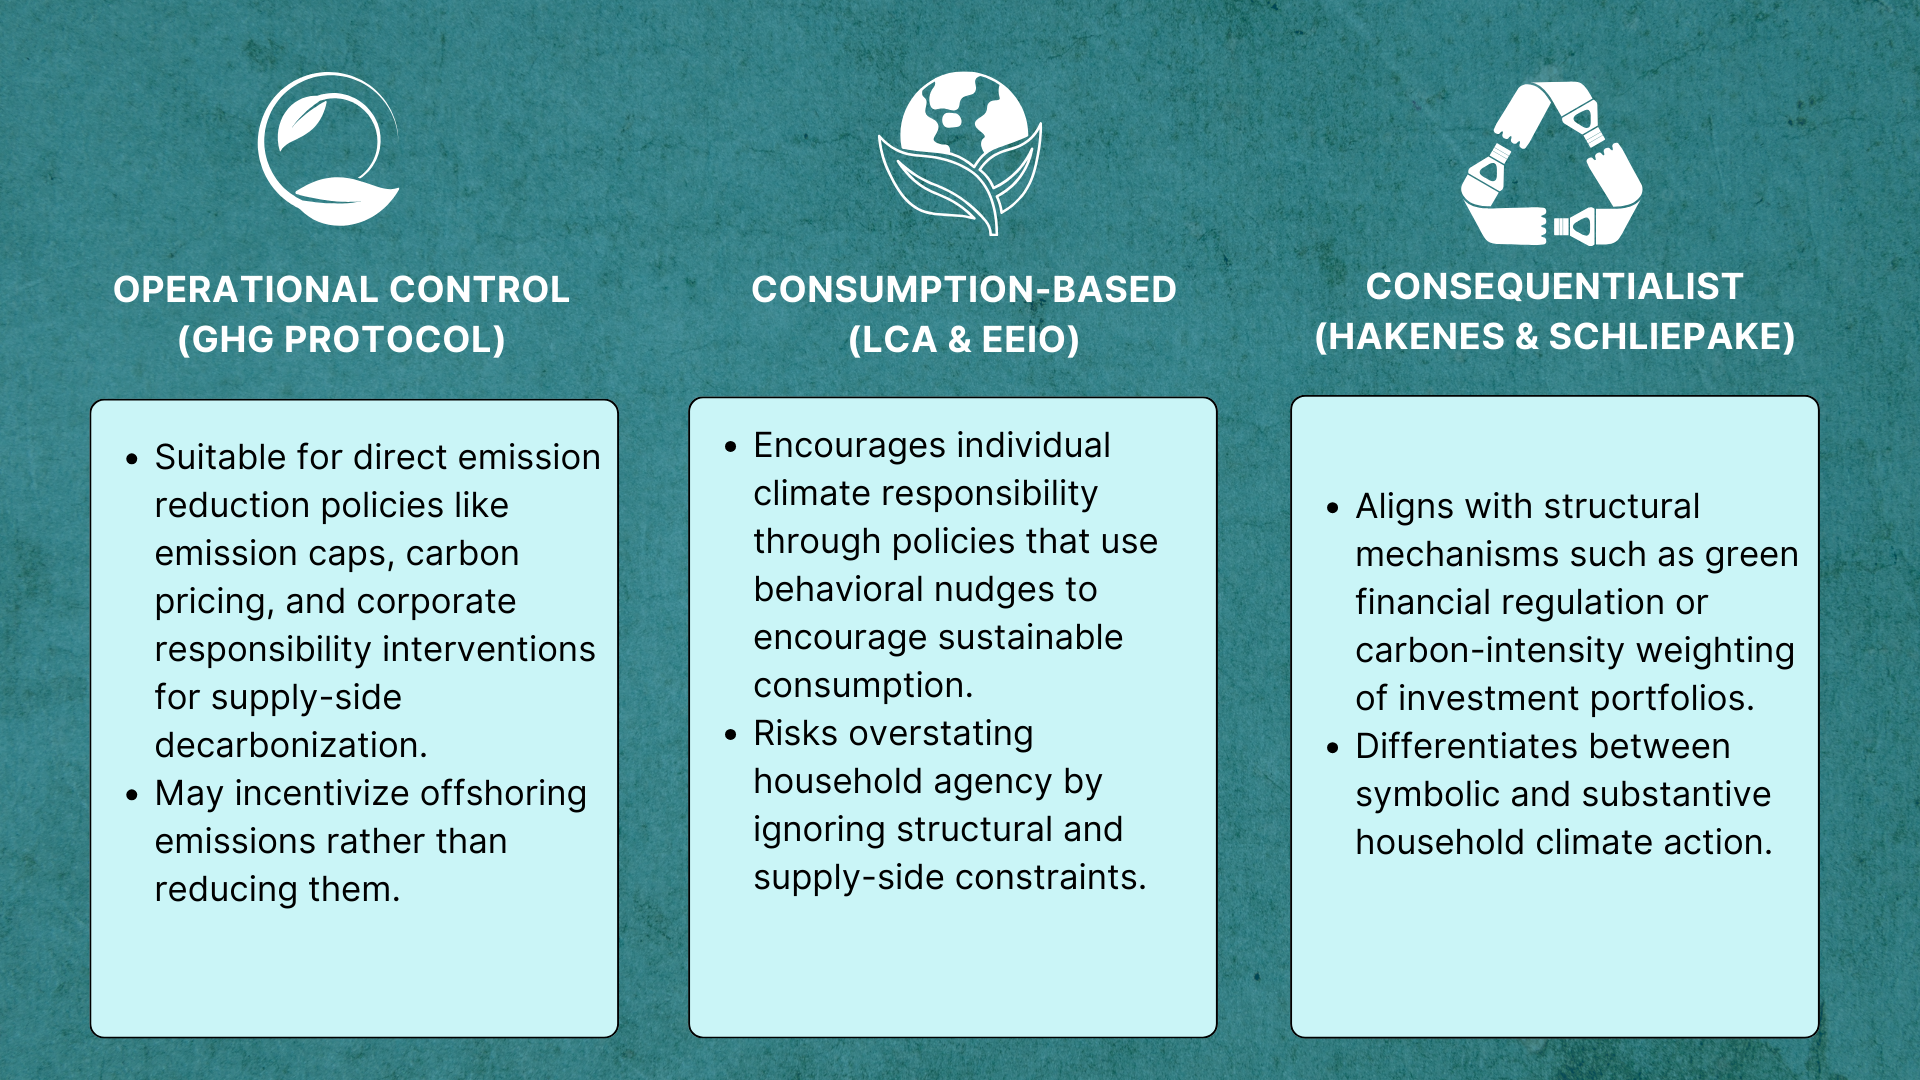
\includegraphics[width=\linewidth]{Policy Implications.png}
\end{figure}
\end{frame}


\begin{frame}{Comparative Analysis of Attribution Principles}
\small
\vspace{-2.5em}
\begin{figure}
  \centering
  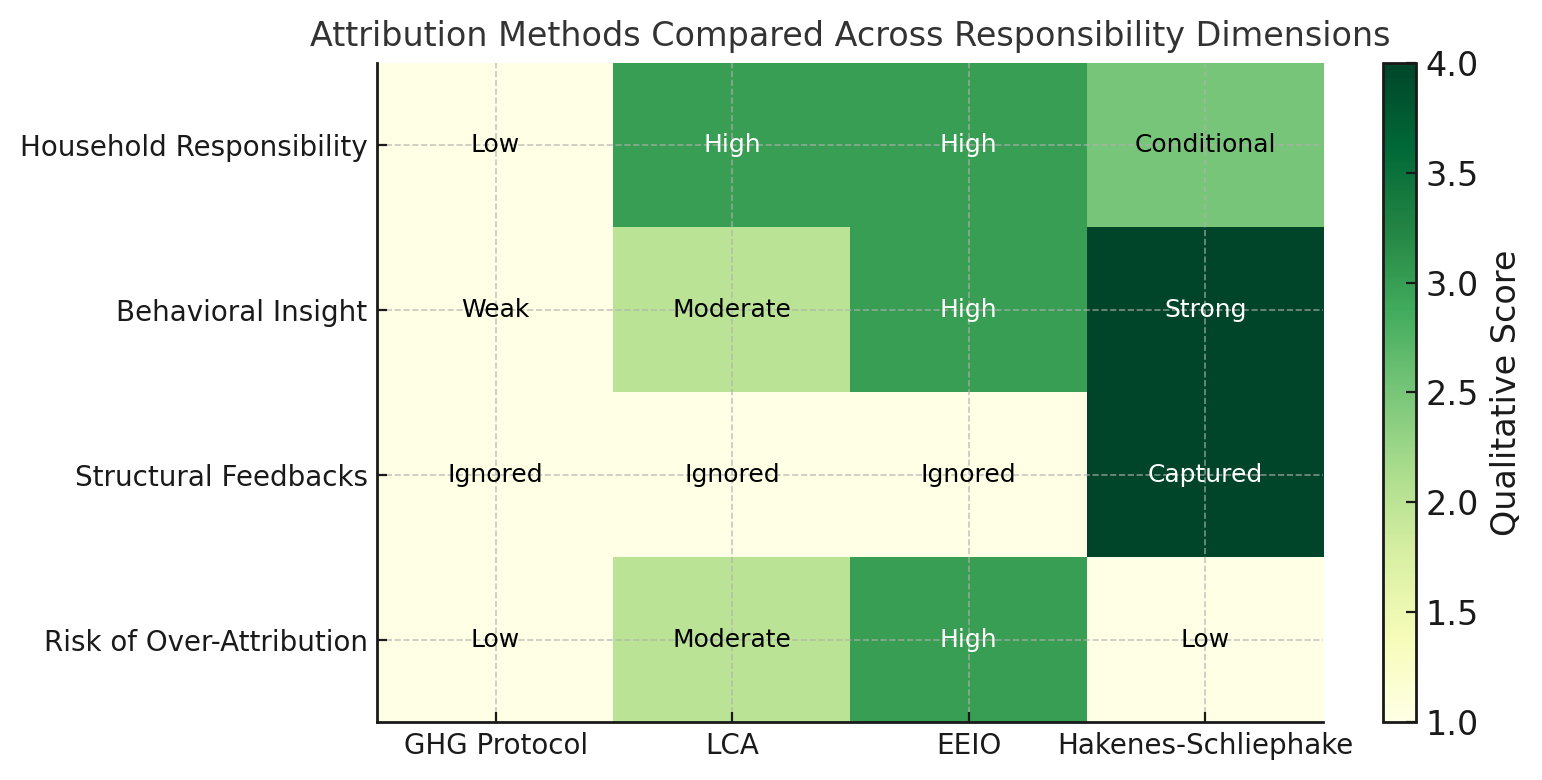
\includegraphics[width=\linewidth]{Heatmap Res.png}
%\caption*{Heatmap comparing estimation methods across household responsibility, behavioral insight, structural feedback, and risk of over-attribution}
  \footnotesize
%\textit{The }
\end{figure}
\footnotesize
%\vspace{0.4em}
%\textbf{Main finding:} Consequentialist attribution (H\&S) uniquely captures systemic feedbacks, avoiding double-counting while grounding responsibility in causal impact.
\end{frame}

\begin{frame}{Household Carbon Footprint Disparities}
  \vspace{-2.0em}
\centering
\pause
\begin{minipage}{0.45\linewidth}
    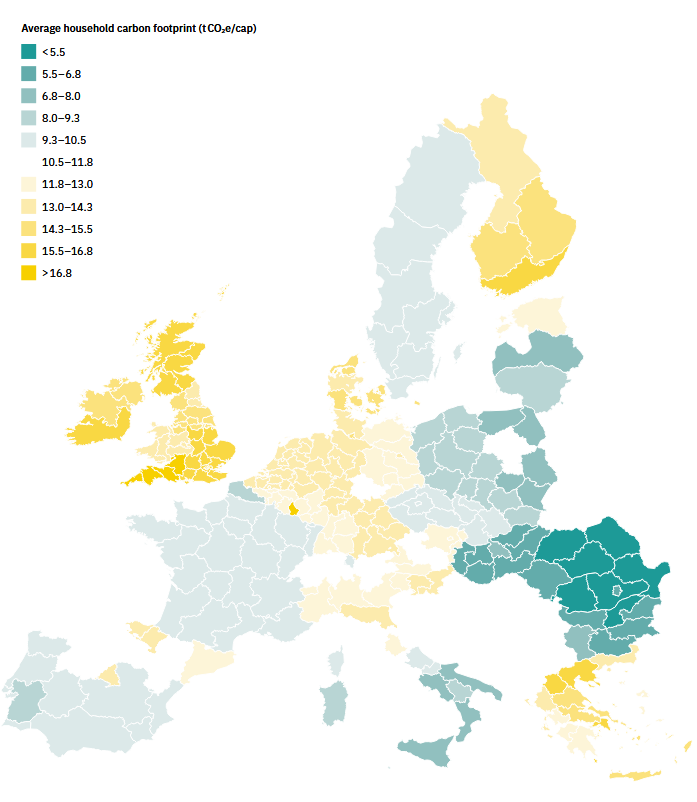
\includegraphics[width=\linewidth]{per capita world emissions.png}
\end{minipage}
\hfill
\pause
\begin{minipage}{0.45\linewidth}
    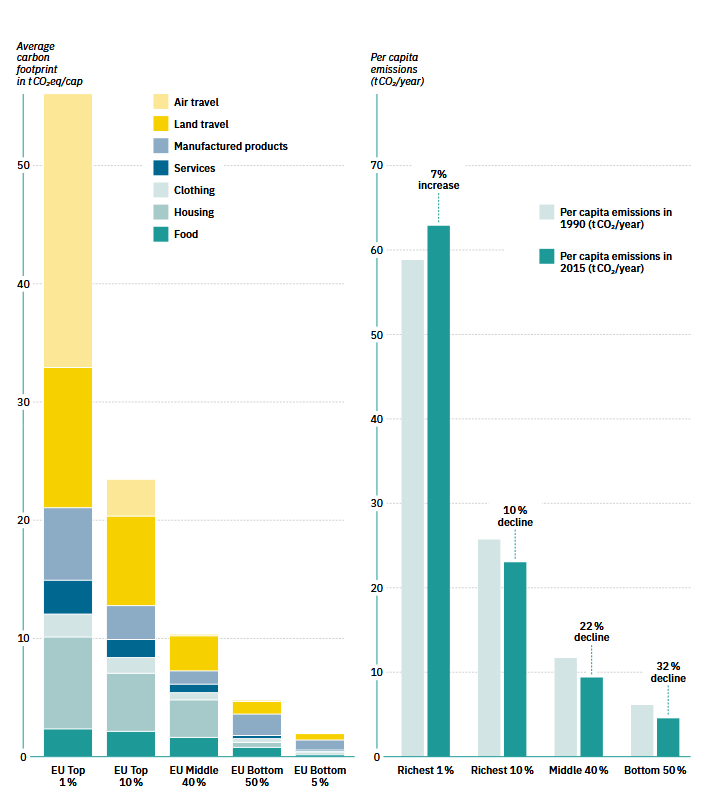
\includegraphics[width=\linewidth]{emission by income.png}
\end{minipage}

\vspace{0.5em}
\footnotesize
%\textit{The heterogeneity in carbon footprints across regions and income groups determines the efficiency and equity outcomes of policy instruments.}
\end{frame}

%---------------------------------------------

\begin{frame}{Comparative Overview of Mitigation Instruments}
\scriptsize
\vspace{-3.0em}
\renewcommand{\arraystretch}{1.15}
\resizebox{\textwidth}{!}{%
\begin{tabular}{p{3.2cm} p{3.3cm} p{3.3cm} p{3.6cm}}
\toprule
\pause
\textbf{Instrument} & \textbf{Methodological Basis} & \textbf{Example Implementations} & \textbf{Features} \\
\midrule

\textbf{Carbon Taxes} & GHG Protocol (Scopes 1–2); EEIO for consumption-based pricing & Sweden: 130+ USD/tCO$_2$; Canada federal backstop; EU Border Carbon Adjustment & Internalises marginal social cost; scalable; regressive without revenue recycling; leakage risk if embedded emissions excluded \\
\addlinespace
\pause
\textbf{Product \& Appliance Standards} & Life Cycle Assessment (LCA); embedded carbon and durability metrics & EU Ecodesign Directive; Japan Top Runner; US Energy Star & Corrects efficiency market failures; harmonisable in trade policy; effectiveness depends on enforcement and affordability \\
\addlinespace
\pause
\textbf{Investment-Based Tools} & General Equilibrium (Hakenes–Schliephake) with EEIO sectoral intensities & EU ETS; California Carbon Allowance; ESG ETFs; Green Bonds & Targets capital allocation to low-carbon sectors; addresses emissions concentration; politically sensitive, data-intensive \\
\addlinespace
\pause
\textbf{Behavioural Interventions} & Behavioural economics; typically outside static carbon models & UK smart meter nudges; diet-shift campaigns; cookstove adoption programs & Low-cost demand adjustment; high social adaptability; persistence and measurement challenges \\
\addlinespace
\pause
\textbf{AI-Enabled Platforms} & Hybrid EEIO–LCA with transaction-level data integration & Moneythor tracker; Svalna app; Klima app & Real-time, marginal behaviour targeting; adaptive feedback; digital divide and privacy governance concerns \\
\bottomrule
\end{tabular}
}
\end{frame}

%---------------------------------------------
%\begin{frame}{Strategic Insights from Comparative Assessment}
%\footnotesize
%\textbf{Key Takeaways:}
%\begin{itemize}
  %\item Attribution logic is endogenous to policy design — \textit{what is measured constrains what can be mitigated}.
  %\item Static, control-based approaches (GHG Protocol) facilitate fiscal and regulatory instruments but understate indirect and imported emissions.
  %\item LCA and EEIO expand system boundaries, enabling product regulation and consumption-based taxation, but risk over-attribution absent behavioural or supply-side constraints.
  %\item Equilibrium models capture inter-market spillovers and capital flows, offering distribution-sensitive interventions, particularly for high-wealth cohorts.
  %\item Behavioural and AI tools bridge micro-level heterogeneity with adaptive policy targeting, but remain weakly institutionalised in formal carbon accounting.
%\end{itemize}
%\end{frame}

%---------------------------------------------
%\begin{frame}{Conclusion: Method–Instrument Alignment}
%\footnotesize
%\textbf{Synthesis:}
%\begin{itemize}
  %\item No single instrument is universally optimal — efficiency, equity, and political feasibility trade-offs are shaped by the underlying attribution framework.
  %\item Integration across methods is essential: \textit{fiscal} (tax), \textit{technological} (standards), \textit{financial} (investment), and \textit{behavioural} levers target distinct channels of household emissions.
  %\item Economically coherent design requires aligning price signals, regulatory standards, and behavioural incentives within the structural constraints revealed by the chosen model.
%\end{itemize}
%\vspace{0.5em}
%\textit{Implication for policy:} Incomplete or mismatched attribution undermines both cost-effectiveness and distributional legitimacy.
%\end{frame}
%---------------------------------------------



\begin{frame}{Optimal Mitigation Portfolio}
\footnotesize
%\begin{itemize}
  %\item \textbf{Attribution methods determine instrument choice:}  
   % \begin{itemize}
    %  \item GHG Protocol $\rightarrow$ direct price signals (carbon taxes, fuel levies).
      %\item LCA $\rightarrow$ product-level regulation (standards, eco-design).
      %\item EEIO $\rightarrow$ consumption-based taxes, trade adjustments.
      %\item General equilibrium $\rightarrow$ capital market instruments.
      %\item Behavioural/AI $\rightarrow$ adaptive, personalised demand-side measures.
   % \end{itemize}
  %\item \textbf{Core trade-offs:}  
   % Taxes = allocatively efficient but potentially regressive.  
   % Standards = technology-forcing, risk of exclusion.  
   % Investment tools = target high-emission wealth segments, politically sensitive.  
  %  Behavioural = socially embedded, hard to monetise.  
  %  AI = granular and dynamic, constrained by digital equity.
 \textbf{Strategic implication:}  
    No single instrument optimises efficiency, equity, and political feasibility.  
    An optimal portfolio integrates complementary tools, each grounded in the correct attribution logic, to maximise mitigation while maintaining fairness and public acceptance.
%\end{itemize}
\end{frame}

\begin{frame}{Policy Recommendations}
  \pause
  \vspace{-2.5em}
\begin{figure}
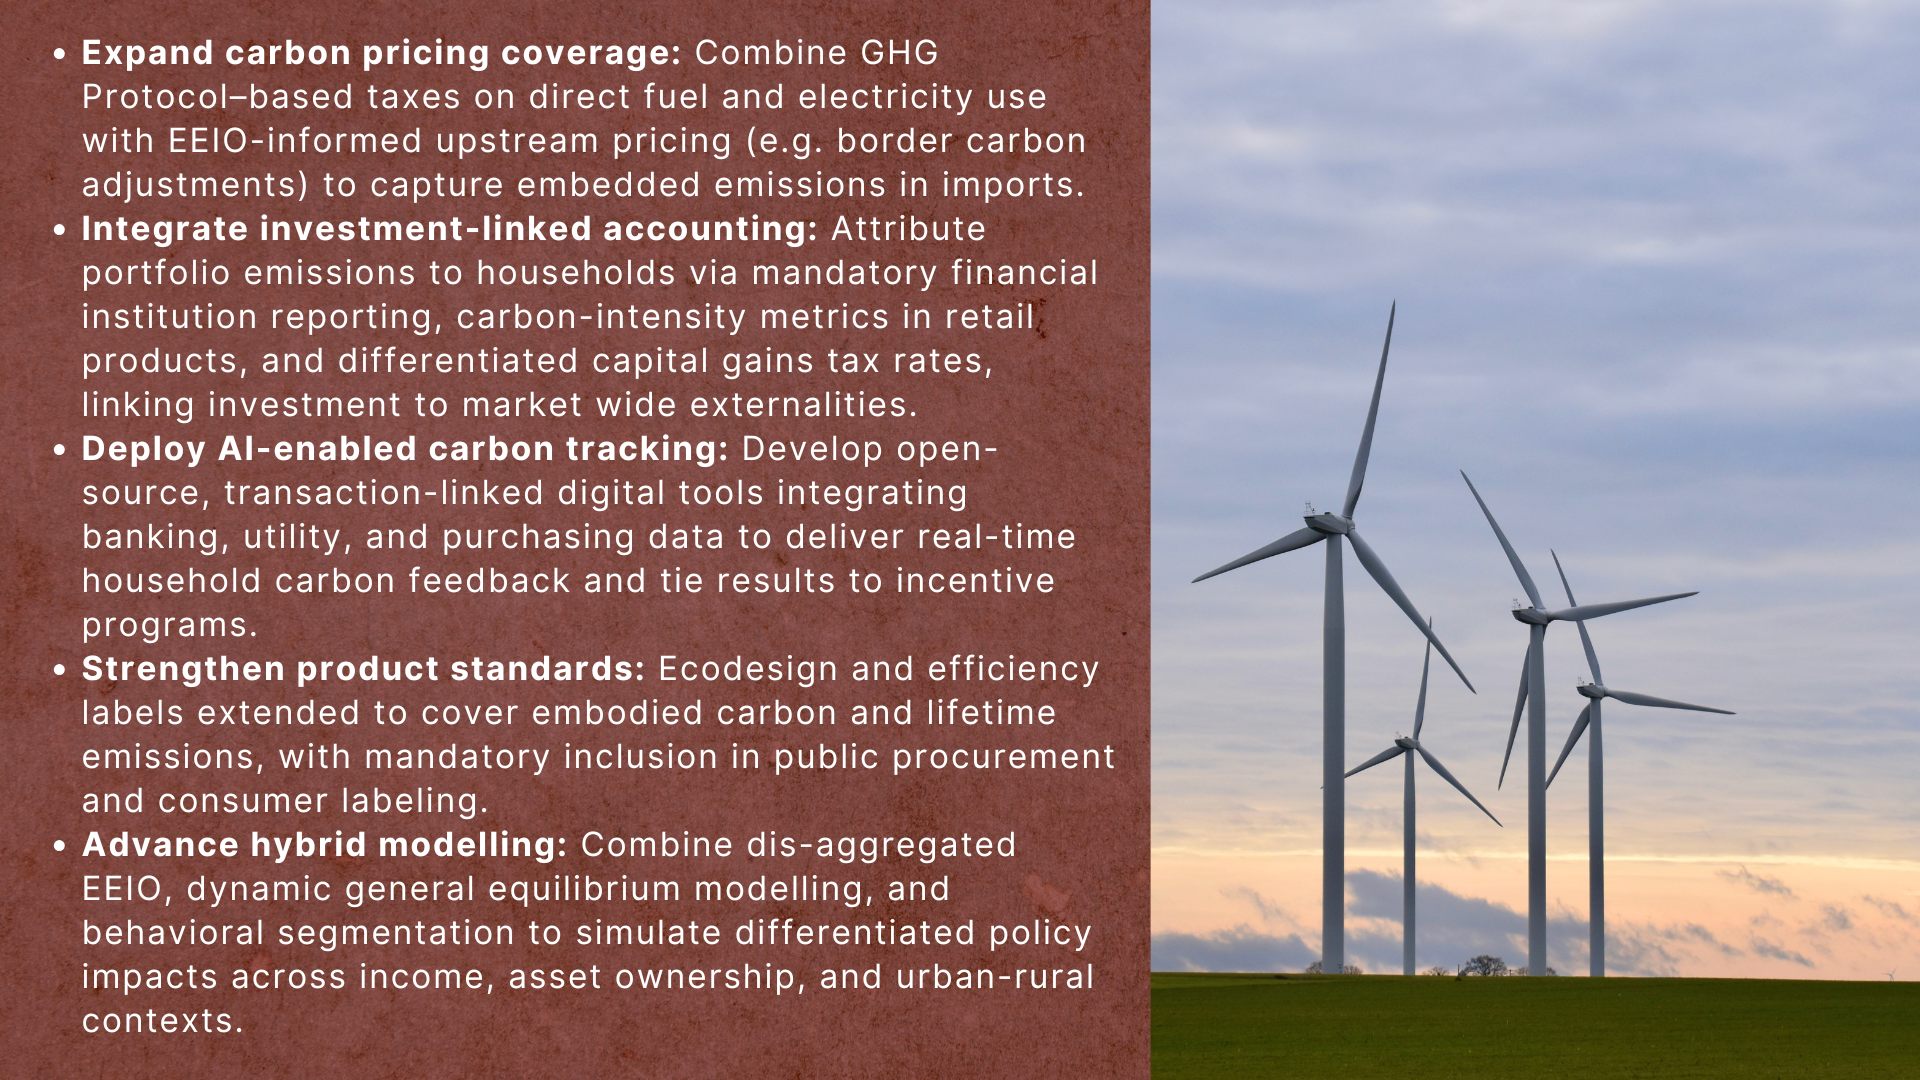
\includegraphics[width=\linewidth]{Policy Recommendation.png}
\end{figure}
\end{frame}

\section{Conclusion}
\begin{frame}{Conclusion}
  \vspace{-2.5em}
\footnotesize
\begin{itemize}
\item Household carbon footprint estimates vary widely depending on the attribution framework, affecting both magnitude and perceived household responsibility.
\pause
\item GHG Protocol and LCA yield lower household carbon footprints by focusing on immediate consumption and energy use, whereas EEIO and equilibrium models capture broader supply chain and financial market impacts.
\pause
\item Each method naturally supports different instruments (e.g., GHG Protocol → energy pricing, LCA → product and appliance standards, EEIO → upstream intervention, border carbon adjustment, equilibrium models → investment-based interventions).
\pause
\item Overall, the study concludes that household decarbonization strategies must be methodologically consistent, equity sensitive and operationally scalable.    
\end{itemize}
\begin{itemize}
  \pause
\item \textbf{Limitations and future work: }This analysis uses stylized data, a static equilibrium model, and omits behavioral heterogeneity; future research should integrate microdata, dynamic modelling, and machine learning for digital tracking tools.
\end{itemize}
  \end{frame}

  \begin{frame}{}
  
\begin{figure}

\includegraphics[width=\linewidth]{Thank you 2.png}
\end{figure}
\end{frame}
\end{document}


